\documentclass[12.5pt]{report}
\usepackage[a4paper,margin=3cm,footskip=1cm]{geometry}
%\usepackage[cm]{fullpage}
\usepackage{color}
\usepackage{graphicx}
\usepackage{amsmath}

\usepackage{hyperref}

\title{\textbf{Society in simulation\\
Cooperation and bargaining behaviors.}}
\author{}
\date{}
\begin{document}

\begin{titlepage}

\newcommand{\HRule}{\rule{\linewidth}{0.5mm}} 

\center 
\textsc{\LARGE Doctoral Thesis}\\[.5cm] 
\includegraphics[scale=.09]{/home/chi/logou.png}\\[1cm] 
\textsc{\LARGE University of Trento}\\[.4cm] 
\textsc{\Large School of Social Sciences}\\[1cm]
%\textsc{\large Minor Heading}\\[0.5cm] 

%\includegraphics{/media/FUN/tesi/trento.jpg}\\[1cm] 
 
%\HRule \\[0.4cm]
{ \large \bfseries Doctoral School in Economics and Management\\Sociology and Social Research\\Local Development and Global Dynamics}\\[3cm]

\textsc{\Huge Society in simulation}\\[.5cm]
\textsc{\huge Cooperation and bargaining behaviors.}\\[.5cm]

\emph{a dissertation submitted to the doctoral school of economics and management
/ sociology and social research / local development and global dynamics in
partial fulfillment of the requirements for the Doctoral degree (Ph.D.) in
Economics and Management }\\[5cm]

%\HRule \\[1.5cm]
\textsc{\Large Linh Chi Nguyen}\\[.5cm]

{\large \today}\\[5cm]

\begin{minipage}{0.4\textwidth}
\begin{flushleft} \large
\textbf{Advisor:}\\
Professor Edoardo \textsc{Gaffeo} 
\end{flushleft}
\end{minipage}
~
\begin{minipage}{0.4\textwidth}
\begin{flushright} \large
\textbf{Doctoral Committee:} \\
Professor X \textsc{ } 
\end{flushright}
\end{minipage}\\[4cm]



\vfill 

\end{titlepage}
\maketitle
\tableofcontents


\chapter*{Abstract}

This piece of work tracks and describes the evolution of a simulated population playing a certain repeated game in a pair matching fashion. The algorithm is a dynamical process aiming to select the fittest strategy. However, since the strategy space is vast, there exists multiple rest points of the dynamics. By adding some stochastic factor (i.e. the dynamics trembles), the population is likely to cycle among these rest points. A rest point of a dynamics is a weaker concept than a Nash equilibrium point. I would use both of these concepts. The general understanding is that if we calibrate the preference of the player, some qualitatively different equilibria emerge. If we fine tune the selecting dynamics, some equilibria would be more stable than others.\\

However, this work goes deeper into the population for further information. By varying the individual level of patience, I describe how much cooperation one can expect at the macro level when one makes changes at micro level. I then characterise the strategy that sustains cooperation in these periods. For the bargaining behavior, the society also shows different macro patterns at different micro-level patience of the individual. If we are to take the interpretation that society would go through equitable-share phase and unequitable-share phase, I would characterise the strategy in these corresponding periods.\\

For a brief statement of the result, the more patient the individuals are, the better chance and more varieties the society can get at choosing cooperation. It is not necessarily either full cooperation or full defection. There are certain periods holding a half-heartedly cooperative mode.\\

For the bargaining society, the whole picture is richer because the underlying game has more strategies. Claiming fair and square is the obvious and simplest way. 50-50 division is a desirable outcome. However it is (unfortunately or not) not the only way reality can logically turn out because all the deviations out of that mindset, as would be shown later, occurs naturally from the assumption of individual's fitness. These deviations are due to the struggles to gain advantage in the bargaining process. It wastes resources because if the pie is failed to be shared or if there is still something left on the table, it is considered wasteful resources. However, as a matter of fact, negotiations break down and destructive forces exist. They also take many diverse forms. Regarding the patience level of the individual, I suggest that the higher willingness to wait rationalise a new kind of strategy that increases the chance negotiations break down, resources wasted. These newly stable state involves mechanisms such as aggressive claims, prolonged shows of strength, occasional probing and ready retaliations. 

In my simulation, the character that sustains usually takes the form of a strategy that is provocative initially but retreats to modesty after. It can also occasionally probe. Otherwise the society can hold a mixture of strategies that alternate, flexible, testing and yielding if necessary. Apart from what happens in the inefficient periods, I also am curious about what kinds of strategy that would trigger and facilitate the transitions between equitable and non-equitable phases. In details, what character presences at the brink of collapse of the 50-50 division, what makes it half way, and what makes it raise again etc.\\


Keywords: bargaining, repeated game, simulation

\chapter*{Acknowledgements}

I thank School of Social Sciences, University of Trento for the fund, the facility and the administrative support. Especially la BUC, an efficient and artful library.\\

I thank professor Edoardo Gaffeo, and the Board of Sciences overlooking PhD students, for the effort they committed.\\

I thank Matthias Felleisen and his team for the advision.\\

This PhD thesis has gone through many redirections. It benefits gratefully from encountering with fascinating characters along the way. In this final version, I am sorry for the undetected obsolete beliefs. The detected ones are corrected.\\

\chapter*{List of abbreviations}

PD: Prisoners' Dilemma

NE: Nash Equilibrium

ESS: Evolutionarily Stable Strategy

EGT: Evolutionary Game Theory

NDG: Nash Demand Game

NBS: Nash Bargaining Solution\\

\listoffigures
 
\listoftables

\chapter{Introduction}
\section{The context}
\subsection{Game theory: the modern chapter}

Game theory officially started with von Neumann and colleagues amid the war. Just as anything born on the battlefield, this animal carries a certain spirit.\\

The essence of a game is a small scale situation involving "distinct sets of interests". Decision theory involves only one individual's interest. The individual is to maximize her function of utility. The market, on the other extreme, is a situation so large that the individual's action would have no effect. Game theory, as von Neuman points out, involves at least 2 parties and the actions made by these parties affect others. So my utility maximization function includes my and others' actions. I have to think of what the others do and vice versa. The pull and push create a fascinating dynamics.\\

The root of it is a non-cooperative two-person zero-sum game. von Neumann's minimax method and Nash's fixed point based method coincide in giving the solution. From there, however, von Neumann continues to develop it into the theory of cooperative n-person constant-sum game and Nash develops it into the theory of non-cooperative n-person non-constant-sum game. Von Neumann made an attempt to prove that all n-person game then can be reduced to 2 person game and non-cooperative game can be reduced to cooperative game by introducing collusion with Nature. Nash, too, attempted to unify these two branches. Despite the effort, these two branches has continued to harbour and spawn qualitatively different discussions. Since the 50s, Nash's lineage enters a new phase in which we try to refine the Nash equilibrium set. Major milestones are set among the 80s. Since then game theory starts to diffuse horizontally, the results are widely interpreted to other fields. \\

The way we represent strategies also create diverse development paths. The normal form game and the sequential game. These two branches analyse and interpret equilibria in different angles and none can be reduced into the other.\\

To briefly conclude, game theory is a framework to analyse conflicting situations by capturing the essence of conflict into a stylised game with strategies for players. From there we are able to take advantage of mathematical tools to lead the analysing process further. At the end, we interpret the mathematical abstractions back into the original social problem.

\subsection{On simulation and algorithm}
In the repeated game, the strategy space becomes vast which makes it difficult to solve the problem analytically. This motivates me to run simulations on the matter. Each simulation run starts with a population of N agents (usually N = 100). One simulation run can be 500000 cycles, usually more. In the initial population, each agent is assigned one strategy. In each cycle, there are 3 phases: matching phase, learning phase, and mutation phase. In the matching phase, agents are matched randomly in pairs and they execute their assigned strategy to play the game. The resulting payoff then is used to calculate fitness for each agent. The way it is calculated would be discussed further below. In the learning phase, a percentage of the population is allowed to learn. They observe the whole population and choose accordingly the strategy they want to use in the next cycle. The set up is made in such a way that the strategy with higher payoff is more likely to be chosen. Hence the better strategy proliferate at the expense of the poorly performed one. In its mathematical limit, this process is a differential equation. In the mutation phase, a small percentage of the population is allowed to modify their strategy randomly.\\

The learning process is to select the fittest in the current pool and the mutation process is to keep adding varieties into the selection pool. The rationale is that if we run the simulation long enough, we can sufficiently cover the strategy space in order to have interesting and confident result.\\

If we are dealing with the one shot game, the number of strategies is typically 2 or 3. The famous Prisoner's dilemma has 2 strategies: to cooperate or to defect. This makes it easy to calculate analytically the situation. The repeated game, however, has a very large number of strategies. For example, if we repeated the PD for 10 rounds, in each round, a player has 2 possible actions: to cooperate or to defect. Then the number of strategies for the game is 2 to the power of 10. One strategy can be that I cooperate for the whole 10 rounds. Another is that I cooperate for 9 rounds and defect in the last. This makes it difficult to solve the problem by calculation.

\subsection{On mathematical foundation}
Selecting among equilibria requires a certain process. One of those is a replicator dynamics (which is a vector field with immediate interpretation in physics). Underlying those is differential equations. With some added perturbation (the dynamics is trembling), the population may not rested forever in one equilibrium but may visit different equilibria from time to time. Some equilibria may be superior to others, in the sense we dear to add. For example, one may be more fair. But the stability of each does not depend on the adjective we use to describe it. It depends on how large is its basin of attractions, or after settling down how vulnerable it is (i.e. how easy it is to be perturbed out into the basin of another attractor).

\section{The problem}
Currently game theory is in a natural state of diffusing to broader audience. The challenges then would be to develop it deeper and diffuse it better. For the depth of non-cooperative game theory branch, since Nash develops the Nash equilibrium concept hence naturally posing the question to refine the Nash equilibrium set, there are several major equilibrium selection methods developed. But the problem is still wide open. The natural selection process is just one attempt to do so, with no sight of coming any closer to the truth, we are as much as we were in the 80s. Huge jumps in the evolutionary process do come, though. Even if the periods between those are far and tiring, they do punctuate their arrivals.\\

On the other hand, the diffusing process is promising. This work is one part of this movement in the sense that it incorporates simulation and evolutionary algorithm into game theory.

\section{The solution}
I run simulation of some repeated games, and it would show that the population cycles through stable states. I would characterise these stable states which are equilibria of the theoretical game. Using these founded equilibria, I attempt to construct the dynamics of the repeated game. I would not exhaust the theoretically infinite space of the game. I only try to provide an interesting take.

\paragraph{What game?}
The first game is a familiar one: the Prisoner's Dilemma. The second game is the Nash Demand Game.

\section{Innovative aspects}
The innovative aspect of my work lies in the clarity of explanation.\\

The first contribution of this work is that I narrate a full investigation into simulations of population playing games. I would provide full technicality of the simulation and the result. Another contribution is that, when called for by the situation, I bridge the technical description back into reality to attempt to make an interpretation. The interpretation is to be treated with caution.\\

\section{Structure of the thesis}
Chapter 1 is the general introduction. Chapter 2 speaks about the past and current state of the literature that this work fits in. Chapter 3 describes the challenges and problems that the literature calls for. Chapter 4 offers my proposed approach in simulating the iterated Prisoner's Dilemma. Chapter 5 gives the simulation results on the iterated Prisoner's Dilemma in details. Chapter 6 offers my proposed approach in the repeated Nash Demand Game. Chapter 7 gives the simulation results. Chapter 8 describes my simulation setting in the iterated Nash Demand Game. Chapter 9 gives the result.  .... Chapter 11 provides comments and comparisons with related work and chapter 12 concludes. 

\chapter{State of the Art}

The literature of computer simulation on population playing game possibly starts with Maynard Smith and Price. In 1973, Maynard Smith and Price published a computer simulation on the logic of animal conflict \cite{maynard2} and another paper on evolution of animal conflicts regarding game theory in 1974. They saw the similarity between Darwin's natural selection and the cultural selection. So they applied survival of the fittest idea on conflicts in animal society, then expanded it to social norms in human society. This was a bridge between biology and economics.\\

In 1979, Axelrod \cite{axel1} ran a computer tournament. Experts from different fields were invited to write computer program (in Fortran or Basic) as a strategy to play the repeated Prisoner's Dilemma. In the tournament, agents would adopt the strategies and play for 200 rounds. Agents were matched with every other agents (i.e. they play the field). The strategy can be probabilistic, so this is a very general tournament. After that, in 1980, he ran a second round of the tournament \cite{axel2}, with the result of the first one fully published to the public. These two tournaments inspired his book in 1984 \cite{axel3}\\

Regarding the repeated game, in 1986 and 1988, Rubinstein use finite state machine to represent strategies in the repeated bargaining game. He made some notable contributions in classical game theory with mathematical calculation on perfect equilibrium and in the complication of the cost of complex machine. It is to be noted that his approach was not simulation. In computing science, finite state machines were due to Mealy 1955 and Moore 1957. And the literature on genetic algorithm (Fogel 1960s-1970s-1980s, Holland 1975, Fisher 1930) was in the "search for intelligence as a composite ability to find optimum in complex environment", substituting heavy calculation of the experimenter by the evolution of the machine.\\

In 1987, Axelrod wrote about genetic algorithm \cite{axel4} and he made a better structured contribution on the iterated Prisoner's Dilemma simulation. He did not use Moore-Mealy machine (finite state machine) as Rubinstein, but he represented the strategy by Markov model. Specifically, the strategy remembered the results of 3 previous rounds, and prescribed a deterministic move for the next. For example, the outcome of 3 previous rounds was CC, DD, CD, then in the next move, this strategy would play D. The memory of the automata was only 3 and the move was determistic, but it already made the number of possible strategies to be cosmically large (somewhere about $3^{70}$).\\

The details of Axelrod 1987's simulation were as follows: 
\begin{verbatim}
- pick 20 strategies randomly as starting point
- match each one against the 8 benchmarks and calculate the weighted average payoff
- determine the offspring number
- regenerate the population by cross-over method (i.e. sexual reproduction)
- add some mutation
- repeat

The game had 151 rounds. Each run had 50 cycles. He ran 40 runs.
\end{verbatim}
In another setting, the strategies are matched against each other, not to the 8 benchmarks. He ran 10 runs.\\

Also in 1987, Boyd and Lorberbaum \cite{boyd,lorb} published that Tit-for-Tat is not evolutionarily stable. They do this by calculation, not simulation. Also, in the theoretical vein, in 1992, Binmore et al. wrote a paper on finite state machine, in the similar vein with Rubinstein of 1986 and 1988. No strategy is evolutionarily stable in the repeated Prisoner's Dilemma, though. The population just cycle among the equilibria.\\

In 1993, Fogel officially used finite state machine in the simulation of repeated Prisoner's Dilemma. He described in details the method.\\

In 1993, Nowak et al. ran simulation on the iterated Prisoner's Dilemma, using strategy as Markov process. His automata had memory one which means that it remembers only the last round. However, it's probabilistic. For example, if the previous round outcome was CC, it plays C with probability 0.5. And he ran very extensive simulation which was much broader and more general than the work of Axelrod. He starts with some strategies, then after the population settling down, he adds some variation and see if it thrives. He claims a new strategy to hold up cooperation in our society: the win stay lose shift. The other name is Pavlov. The strategy is that you start by defecting and if it works, you keep exploiting but if you get punished, you switch to cooperating. He says that Tit for Tat works in the deterministic society but when it comes to probabilistic, the strategy that sustains cooperation is Pavlov.\\

In those years, many books have been written on the subject. In 2004, there is a paper by Axtell, Epstein, Peyton Young (2004) \cite{axtell}. They also investigate the emergence of equilibrium points in the Nash Demand Game using simulation. They use two settings, one has agents with memory which is a sort of repeated game, the other is a sort of one shot game but agent has irrelevant tags (for example, color of their skins). They found that there are three types of stable situations: a fair division, a not-fair but efficient division, a situation of inefficient sharing. However my study is different in the feature that I don't use tag for agents, and the repeated game is set up in a different way from Axtell et al.\\

In 2012, Press and Dyson published some result on the iterated Prisoner's Dilemma, in which the strategy is memory one Markov process. Again, this is from the analytical side, not simulation.\\

What makes running simulations very potential is the fact that there are so many possible technical settings you can use for the simulation. You can run it on spatial structure, you can run it with different level of assortive mating (0 included), you can run it with different number of rounds on the repeated games, you can run with agents with different length of memory etc.


\chapter{The problem}
The problem that the game theory simulation literature is going after is, in general, searching for optima in a vast space. The strategy space of one shot PD has 1 dimension. Let $P_{C}$ be the probability of choosing C then the probability to choose D is $1 - P_C$. If we are dealing with a repeated game of 3 rounds, the number of strategies is $2*2*2 = 2^3 = 8$. The possible strategies are:

\begin{verbatim}

C - C - C  ->  CCC
  \   \ D  ->  CCD
    D - C  ->  CDC
      \ D  ->  CDD
D - C - C  ->  DCC
  \   \ D  ->  DCD
    D - C  ->  DDC
      \ D  ->  DDD
      
\end{verbatim}

The strategy space of this game, hence, has 7 dimension. If we suppose to play the game infinitely, the number of strategies is $2^{\infty}$, the number of dimensions of the strategy space, therefore, is $2^{\infty} - 1$. It is incredible hard to find the optima in such a vast space, therefore, I approach by doing simulation.


\chapter{My proposed approach: Simulation for the iterated PD}

\section{The Prisoner's Dilemma game}

\begin{table}[h!]
\center
\begin{tabular}{l|ccc}
\textbf{PD} & Cooperate & Defect \\
\hline
Cooperate & 3,3 & 0,4 \\
Defect    & 4,0 & 1,1 \\

\end{tabular}
\caption{Prisoner's Dilemma payoff matrix}
\end{table}

\section{Implementation}
\paragraph{Population and Agents}
Starting from a world with many slots, we populate them with agents. The population will be kept fixed and each agent will adopt a strategy/machine to execute when playing the game. A brief definition of agents is that agents do agency: given a strategy, they play by the book until they terminate.

\paragraph{Cycle}
A typical cycle has 3 phases: matching phase, learning (or regeneration) phase, and mutation phase. In the matching phase (Figure 4.1), agents will be matched randomly in pair to play the game for multiple rounds. Their payoff sequence will be collected to calculate the corresponding fitness (i.e. the relative share of each final payoff in the total population payoff). 
\begin{figure}[h!]
 \center
\includegraphics[scale=.55]{/home/chi/Google" "Drive/master-tesi/pic/cycle1.png}
\caption{Matching phase}
\end{figure}
The fitness vector of the whole population will be used in the regeneration phase (Figure 4.2). In the regeneration phase, a small number of agents will be allowed to \emph{learn}. Technically, they randomize over the fitness vector to choose their new strategy. Because the fitness of each strategy is different, a better strategy will be more attractive and it'll be more likely to be chosen hence it'll become more popular at the next cycle. In this way, the strategy that performs better will grow at the expense of the poor doers. 
\begin{figure}[h!]
 \center
\includegraphics[scale=.55]{/home/chi/Google" "Drive/master-tesi/pic/cycle2.png}
\caption{Learning phase}
\end{figure}
In the mutation phase (Figure 4.3), a small number of agents will experiment on their current strategy (mutating). This is to keep adding variety into the selection pool.\\

\begin{figure}[h!]
 \center
\includegraphics[scale=.55]{/home/chi/Google" "Drive/master-tesi/pic/cycle3.png}
\caption{Mutation phase}
\end{figure}


\paragraph{Rationale}

If there is X strategies available in the strategy space and if we start the simulation with a population of X agents holding all possible strategies of the game, then the learning process would be sufficient to single out the fittest survivors given that we run the simulation long enough. To accommodate for the likely possibility of multiple equilibria, we run the simulation many many times to collect the set of different survivors. The winner can be a pure strategy or it can be the population state of a mixed strategy. X, however, is huge in almost any cases, we start the simulation with initial population of N = 100 agents plus using the mutation process. If we do not use the mutation process, the initial population affects the ending result. The mutation process is to keep adding varieties into the selection pool. When doing this, the initial population does not matter. Because the population would keep receiving new strategies, the strategy space coverage would increase gradually. If we run a very long simulation, a good portion of the strategy space would be examined. 

\section{Strategy implementation: Markov chain}

The PD has 4 outcomes for one round: CC, CD, DC, DD.

Here is one strategy using Markov chain in its structure: the deterministic Tit for Tat:

\begin{verbatim}
(
the propensity to cooperate:
- initial round: 1
- after cc: 1
- after cd: 0 
- after dc: 1 
- after dd: 0
)
\end{verbatim}

This one is an almost deterministic Tit for Tat. We call it a probabilistic Tit for Tat.
\begin{verbatim}
(
the propensity to cooperate:
- initial round: 0.99
- after cc: 0.9
- after cd: 0.1
- after dc: 0.95
- after dd: 0.05
)
\end{verbatim}

I adopt another abbreviated version of automaton description:

\begin{verbatim}
                    init  cc  cd  dc  dd 
Always-cooperator (  1  |  1   1   1   1 )
\end{verbatim}

This one starts out by cooperating absolutely, and continues to cooperate absolutely regardless of the previous outcome. It is an always cooperator. Another classic automaton is the always-defector:

\begin{verbatim}
Always-defector   ( 0 | 0 0 0 0 )
Tit for tat       ( 1 | 1 0 1 0 )
Grim trigger      ( 1 | 1 0 0 0 )
Winstay loseshift ( 0 | 1 0 0 1 )
\end{verbatim}

The always-defector starts the game defecting, ends the game defecting and defecting everywhere in between. No outcomes change its behavior.

Tit for tat is the one that starts out cooperating and continues to cooperate as long as the opponent cooperates. Once the opponent defects, it switches to defecting to punish. If the opponent switches back to cooperating again, it also goes back. This one forgives.

Grim trigger is the one that starts out cooperating and continues to do so as long as the opponent does. Once the opponent switches to defect, it switches to defecting and never goes back. It does not forgive, and does not forget.

Winstay loseshift's scheme is simple. It starts out defecting. Then it considers the outcome. If the outcome is benefiting it keeps doing what it was doing. Hence after a CC, it continues to cooperate. After a DC it continues the exploiting behavior. If the outcome is not benefiting it switches the behavior. Hence after a CD, its propensity to cooperate is 0. After a DD, it switches back to cooperating. This one keeps exploiting the opponent if the opponent keeps submitting but if the opponent punishes, it switches back to cooperating.

The mutation would change the probability plausibly, one at a time. For example, if the mutation happens at the propensity to cooperate of currently 0.70, it can raise the propensity up to 1 or it can decrease the propensity down to 0.

\section{Payoff calculation}
Since a match of 500 rounds gives a sequence of 500 payoffs, I use factor $\delta$ as in the bank to calculate the present value of this future-involved sequence. This is a repeated game and we interpret the sequence from round 2 onwards to be in the future. A myopic person has a small $\delta$ which means that how much she considers to get from the 500 round game relies heavily on the first few rounds. After that, even a series of highest possible payoffs would not interest her. She considers high payoffs in the future to be 0 and dismiss them. This kind of person would prefer to get high payoffs in the first few rounds, she would choose the sequence 2 over sequence 1 in the following example:

\begin{verbatim}
sequence 1: 0 0 0 0 4 4 4 4 4 4 4...
sequence 2: 4 4 4 0 0 0 0 0 0 0 0...
\end{verbatim}

On the other end of the spectrum, a person with high $\delta$ is a highly patient person. She can wait for the payoffs in the future or at least she would take them into account. For her, 1 euro of tomorrow worths almost as 1 euro of today. She would prefer sequence 1 over sequence 2 with sufficiently high $\delta$.

There is another interpretation of $\delta$ as continual probability in which the first round is played for sure. At the end of that, a $\delta$ biased coin is flipped, with probability $\delta$ the game continues, and with probability $1 - \delta$ the game stops. 

Mathematically these two interpretation converges but in implementation, regarding the same $\delta$, it is more stable to implement it as discounting factor, which I do here.

I can also run the simulation with the continual probability implementation, the result, though qualitatively similar, is very noisy making it difficult to see the point.

The noise comes from the fact that, for 50 pairs of even the same agent, the numbers of rounds varies greatly even though the continual probability $\delta$ come from the same distribution. For example, let's say we have 10 agents using the same strategy. Since $\delta$ is an independent and random draw, these 10 agents can get to play 10, 100 or 150 rounds which give a volatile payoff despite the fact that they are using the same strategy. Of course, with the law of large numbers, the average payoff should reflect well the merit of the strategy but here we are dealing with small numbers. This volatility is affecting the fitness of a strategy unnecessarily, as in my opinion.

\section{500 rounds}

I usually set the number of rounds to be 500. Because at the maximum $\delta$ = 0.99, the payoff at round 500 would be negligible. I assume that the match can be safely cut off after this threshold. The corollary is that I can still safely assume this to be an infinite match. Certainly one can ask about $\delta$ = 0.9999 but I would say that rounding up to 2 decimals is a reasonable assumption about how the world works. Also, in computing, these imprecise approximations are common (see: floating numbers). They serve reality well.

\chapter{Simulation result : the iterated Prisoner's Dilemma}

\section{Patient players}
I run with the following configurations. The population has fixed N agents, with N = 100. The number of rounds to be played when two agents are matched is 500. The delta to calculate present value of the 500 payoff sequence is 0.99. The learning rate is 10 percent. The mutation rate is 1 percent.\\

$\delta = 0.99$ is very close to 1. This represents a highly patient agent. Then I plot the average payoff of the whole population in each cycle, with two benchmarks. The red line is the state of everybody defecting everybody in every round. The blue line is the state of everybody cooperating with everybody in every round.

\subsection{$\delta$ = 0.99}

\begin{figure}[h!]
\center
\includegraphics[scale=0.3]{/media/FUN/pd-0118/data499/1pic.png}
\caption{One typical run: $\delta$ = 0.99}
\end{figure}

Overall, I have two brief comments. First, with the probabilistic markov chain in the structure of the strategy (i.e. the probability to cooperate tomorrow depends on the outcome of today), the population spends half the time in cooperative mode which is not bad. Another comment is that there different degree of cooperation, ranging from full defection to full cooperation. Let's take a look at a sample run and I would take out automaton from interesting points in the run to see what kind of strategy sustaining different levels of cooperation.

\subsubsection{Simulation 1}
In Figure 5.1, let's see further into 3 points of interest: cycle 10K, 16K and 18K. These 3 points are of interest because they have different degree of cooperation. We can see what mechanism is used to uphold it.

\paragraph{Point 1}

Figure 5.1, cycle 10000, the population is in a moderately cooperative mode. The population mean is around 220. The fully cooperative state has the population mean to be 300. In this state, 100 percent of the population is this automaton:

\begin{verbatim}
( init |  cc   cd   dc   dd  )
( 0.61 | 0.43 0.35 0.97 0.89 )
\end{verbatim}

The propensity to cooperate in the initial round is 0.61 which is optimistic. The propensity to cooperate after both cooperating is 0.43 which shows an urge to betray. The propensity to cooperate after being betray is 0.35 which is an urge to punish. The propensity to cooperate after exploiting is 0.97 which is highly regretful (almost absolute). The propensity to cooperate after both defecting is 0.89 which shows an aspiration to go back to the CC outcome.\\

In general, this automaton wants to try to opposite. If it is cooperating, it has the temptation to go defecting (though not as high as the other way around). If it is defecting, it has a very high desire to go back to cooperating. If it is matched with itself, it generates a lot of (3,3) and some alternating sequence of (4,0) and (0,4).

\paragraph{Point 2}

Figure 5.1, cycle 160000, the population is in a highly cooperative mode. The population mean is around 290. The fully cooperative state has the population mean to be 300. In this state, 100 percent of the population is this automaton:

\begin{verbatim}
( 0.7 | 20.99 0.37 0.77 0.07 )
\end{verbatim}

The propensity to cooperate in the initial round is 0.72 which is optimistic. The propensity to cooperate after both cooperating is 0.99 which is absolute commitment (no temptation). The propensity to cooperate after being exploited is 0.37 showing that betrayal is consequential. The propensity to cooperate after exploiting is 0.77 which is highly regretful. The propensity to cooperate after both defecting is 0.07 which is zero-forgiving.\\

In general, this one is a forgiving Tit for Tat. As reference, here is a Tit for Tat:

\begin{verbatim}
Tit for Tat: ( 1 | 1 0 1 0 )
\end{verbatim}

\paragraph{Point 3}

Figure 5.1, cycle 180000, the population is able to reach a higher cooperative state (almost absolute) than in cycle 160000. It contains the following automaton:
\begin{verbatim}
( 0.72 0.99 0.37 0.77 0.32 )
\end{verbatim}

This is a mutated version of the previous one in cycle 160000. It has a higher aspiration to come back to the utopian vision of a society after seeing the outcome of both side's selfishness. It is a better version of Tit for Tat. Although its punishing tool becomes less effective on fully defective strategy (i.e. the one that insists on defective).

\subsubsection{Simulation 1 continued}

In Figure 5.2, I would look into 5 points of interest: cycle 10K, 85K, 100K, 150K, 165K. I pick the first 4 points because they represent different levels of cooperation. The last one is the one that marks the collapse of fully cooperative mode. The population goes from full cooperation to full defection in a very fast manner.

\begin{figure}
\center
\includegraphics[scale=0.3]{/media/FUN/pd-0118/data499/2pic.png}
\caption{One typical run: $\delta$ = 0.99 the sequel}
\end{figure}

\paragraph{Point 1}

Figure 5.2, cycle 10000, the population continues to enjoy a similar highly cooperative mode. The automaton is a bit different:
\begin{verbatim}
( 0.77 0.99 0.44 0.55 0.32)
\end{verbatim}

The propensity to cooperate in the initial round is 0.77 which is optimistic. The propensity to cooperate after both cooperating is absolute commitment. The propensity to cooperate after being exploited is 0.44 which is as coin flipping. It is not seeking punishment, but also not taking the betrayal easy. The propensity to cooperate after exploiting is 0.55 which is as coin flipping. This shows some temptation to continue exploiting. The propensity to cooperate after both defecting is 0.32 which is hopeful to some degree.\\

In general, this automaton is a so-much better version of Grim Trigger.

\begin{verbatim}
Grim Trigger: ( 1 1 0 0 0 )
\end{verbatim}

A Grim Trigger starts out to cooperate and continues cooperating as long as the opponent is doing so. Once the opponent defects, it switches to defecting forever. It does not forgive, does not forget.

\paragraph{Point 2}

Figure 5.2, cycle 850000, the population mean is around 230. The absolute cooperative mode has the mean of 300. In this mode, it contains the automaton:
\begin{verbatim}
( 0.53 0.99 0.24 0.04 0.16 )
\end{verbatim}

This one flips a coin in the first round. It absolute commits to the utopian society. After being exploited, it provides high consequence, but still offers some tolerance with the propensity to cooperate being 0.24. After exploiting the other, it shows absolute intention of continual defection. After the outcome of both defecting, it has propensity to cooperate of 0.16 which is highly defective.\\

In general, it is a Grim Trigger with some margin. If being matched with itself, it creates a long streak of rewards (3,3) then a less longer streak of punishment (1,1) then back to a rewarding society. There is not much alternating.

\paragraph{Point 3}

Figure 5.2, cycle 100000, the population mean is about 290. The absolute cooperative mean is 300. The population consists of the automaton:

\begin{verbatim}
( 0.53 0.99 0.88 0.04 0.16 )
\end{verbatim}

This one flips a coin to enter the game. If it cooperates, it continues to do so regardless of the other. If it defects, it continues to do so. It certainly provides some leeway to cushion the betrayals and come-backs. If it is a deterministic one it would be (1 1 1 0 0) which is someone living up to its own standard.

\paragraph{Point 4}

An evolved version of this is in cycle 150000:
\begin{verbatim}
( 0.53 0.99 0.93 0.04 0.53 )
\end{verbatim}

If this one cooperates, it is very committing to its own standard. But after the outcome of effective exploiting, it absolutely intents to continue the exploiting. After both being punished, it flips a coin to hopefully cooperate.\\

This one is able to maintain an almost absolutely cooperative mode, but soon the population gets invaded by a highly defective one. 

\paragraph{Point 5}
In cycle 165000, it is a Defector:

\begin{verbatim}
( 0.5 0.04 0.13 0.04 0.15 )
\end{verbatim}

\subsubsection{Simulation 1 continually continued}

\begin{figure}[h!]
\center
\includegraphics[scale=0.3]{/media/FUN/pd-0118/data499/3pic.png}
\caption{One typical run: $\delta$ = 0.99 the 2 sequel}
\end{figure}
I continue to run this after the first two because the first two runs demonstrate how the society can go from low cooperative mode to fully cooperative mode and then how it collapses. This run is to show how it raises again. Hence I would pick two points of interest, the one before it raises and the one after: cycle 70K and 80K.

\paragraph{Point 1}


Figure 5.3 cycle 70000, the population mean is 260. The absolute cooperation gives the mean of 300. The population is full of this automaton:
\begin{verbatim}
( 0.99 0.96 0.07 0.77 0.54 )
\end{verbatim}

The propensity to cooperate in the first round is absolute. The propensity to cooperate after both cooperating is absolute commitment. The propensity to cooperate after being betrayed is absolute zero. The propensity to cooperate after exploiting is 0.77 which shows a margin of continual temptation. The propensity to cooperate after both being defective is a coin flipping which is neutral (i.e. neither seeking vengeance nor being forgiving).

\paragraph{Point 2}

After 10000 cycle more, a mutated version of the above automaton lifts the whole population up to a better cooperative mode:
\begin{verbatim}
( 0.99 0.96 0.07 0.77 0.99 )
\end{verbatim}

The propensity to cooperate after a punishment is absolute.

\subsubsection{Simulation 2}

Before moving on to reduce the patience level of the individual, I report here another sample run of the same settings. It is easy to replicate the two brief comments I make at the beginning of this section: the population spends half the time in cooperative mode and cooperation has its degree.

\begin{figure}[h!]
\includegraphics[scale=0.15]{/home/chi/Downloads/pd-0118/199pic.png}
\includegraphics[scale=0.15]{/home/chi/Downloads/pd-0118/299pic.png}\\
\includegraphics[scale=0.15]{/home/chi/Downloads/pd-0118/399pic.png}
\includegraphics[scale=0.15]{/home/chi/Downloads/pd-0118/499pic.png}
\caption{$\delta = 0.99$ Another run of 2 000 000 cycles}
\end{figure}

\subsection{$\delta$ = 0.95}
In this simulation I reduce the patience level of the individual from $\delta = 0.99$ to $\delta = 0.95$. This changes the payoff calculation. If the player is to fully cooperate and be rewarded, she gets 3 in all rounds. However, the final payoff is scaled back to 60, instead of 300 as in the previous simulation. The benchmark payoff changes, other things remain the same.

\begin{figure}[h!]
\includegraphics[scale=0.12]{/media/FUN/pd-0118/data595/1pic.png}
\includegraphics[scale=0.12]{/media/FUN/pd-0118/data595/2pic.png}
\includegraphics[scale=0.11]{/media/FUN/pd-0118/data595/3pic.png}
\caption{One typical run: $\delta$ = 0.95. a b c.}
\end{figure}

We can see that the population climbs to a middle situation of cooperation, then climbs up to the full cooperation and maintains that situation for very long time. At some point, it collapses completely and the defective mood also stays for long. However, at some other point, the population payoff raises again.\\

\subsubsection{Simulation 3 a}

I would pick out some points of interest. The first one is when the population is at the moderately cooperative mode. The second one is when it reaches almost full cooperation. The third one is when it reaches for even higher and the last one is when it drops a little bit.\\

\paragraph{Point 1}

In figure 5.5a, cycle 30000, the population mean is at 45. The absolutely cooperative population has mean of 60. 100 percent of the population is this automaton:

\begin{verbatim}
( 0.36 0.99 0.09 0.39 0.26 )
\end{verbatim}

It starts out defecting, and if a defection happens, the probability to come back cooperating is low, but not zero. After a situation of both cooperating, it commits absolutely to the utopian society.

\paragraph{Point 2}

At cycle 70000, the population achieves the mean of absolute cooperation (around 60). 100 per cent of the population is this automaton:
\begin{verbatim}
( .81 .99 .09 .98 .98 )
\end{verbatim}

It is highly cooperative in most scenarios. Except for the outcome of being betrayed.

\paragraph{Point 3}

At cycle 100000, the population mean is the same but the mechanism sustaining cooperation is a different automaton:

\begin{verbatim}
( .85 .99 .09 .07 .98 )
\end{verbatim}

It is a good Pavlov (Win stay Lose shift). Here is a Pavlov:

\begin{verbatim}
( 0 1 0 0 1 )
\end{verbatim}

A Pavlov starts to defect and keeps doing so if defection is benefitial (for example, after the outcome (D,C)). If cooperation is benefitial (after the outcome of (C,C)) it also keeps cooperating. When its action is not benefitial, for example when it is betrayed (C,D) or when both being punished (D,D), it switches behavior (from C to D and from D to C, respectively).

\paragraph{Point 4}

At cycle 120000, the automaton evolves into an even better one: the propensity to cooperate in the first round is 0.99.

\begin{verbatim}
( .99 .99 .09 .07 .98 )
\end{verbatim}
With these kinds of automaton, the payoff sequence they produces consists of long streaks of (3,3) because after a (3,3) the propensity to commit is absolute. And if a (1,1) happens the propensity to come back to (3,3) is absolute.

\subsubsection{Simulation 3 b}

In this run we have 3 points of interest, the one in full cooperative mood, the tiny window where the payoff drops in half, and the one where it drops completely to defection everywhere.\\

\paragraph{Point 1}
Figure 5.4 b, cycle 90000, the population is full of this automaton:

\begin{verbatim}
( .01 .99 .38 .66 .98 )
\end{verbatim}

The propensity to cooperate in the first round is zero. The propensity to cooperate after a (C,C) is absolute. The propensity to cooperate after being betrayed is 0.38 which is tolerating. The propensity to cooperate after betraying is 0.66 which has a margin of continual temptation. The propensity to cooperate after being punished is absolute.

\paragraph{Point 2}

5000 cycles after, the population mean drops in half (to 40), because of the invasion of a mutated version:

\begin{verbatim}
( .01 .11 .38 .66 .98 )
\end{verbatim}

This one is mostly the same, except for the propensity to cooperate after a (C,C) dropping to 0.11. Hence if it is matched with itself the payoff sequence alternates among (4,0), (0,4), (1,1) and (3,3). However, it invades the previous one because if it is matched with the previous one, it is able to exploit and enjoy lots of (0,4) rounds. The previous one, after being exploited, has propensity to cooperate of 0.38 which is a bit tolerating.

\paragraph{Point 3}

In 5000, the population mean drops to base line (absolute defection). The population is full of this automaton:
\begin{verbatim}
( .01 .11 .38 .66 .1 )
\end{verbatim}

This one mutates the propensity to cooperate after a (D,D) by dropping it from 0.98 to 0.1. Hence it invades the previous population. From this cycle onward, it does not pay to be tolerating anymore, hence the other propensity also drop resulting in the further decrease of the population mean.

\subsubsection{Simulation 3 c}
Let's take 2 points of interest: the one at full defection and the one on the high level.

\paragraph{Point 1}

In Figure 5.4, picture c, cycle 130000, the population achieves the mean of 50. The fully cooperative mean is 60. The population is full of Tit for Tat:
\begin{verbatim}
( .78 .97 .04 .94 .04 )
\end{verbatim}

The propensity to cooperate in the first round is 0.78 which is optimistic. The propensity to cooperate after the opponent cooperating is 0.97 and 0.94 which is absolute. The propensity to cooperate after the opponent defecting is 0.04 and .04  which is zero.

\paragraph{Point 2}

At 150000 cycle, where the mean is almost 60, the population is full of the following automaton:
\begin{verbatim}
( .78 .98 .91 .94 .04 ) 
\end{verbatim}

This automaton is highly optimistic except for the case of both defecting. In that case, the propensity to cooperate is 0.04 which is hopeless.

\subsection{$\delta$ = 0.9}

\subsubsection{Simulation 4}
I report here simulation on lower level of patience. The 2 brief comments are in place, however, the population spends less time in cooperative mode. It shows a decrease in cooperation at society as individuals lose sight of the long run. I would say it drops to 30-40\%.

\begin{figure}[h!]
\includegraphics[scale=0.15]{/media/FUN/pd-0118/data690/1pic.png}
\includegraphics[scale=0.15]{/media/FUN/pd-0118/data690/2pic.png}\\
\includegraphics[scale=0.15]{/media/FUN/pd-0118/data690/3pic.png}
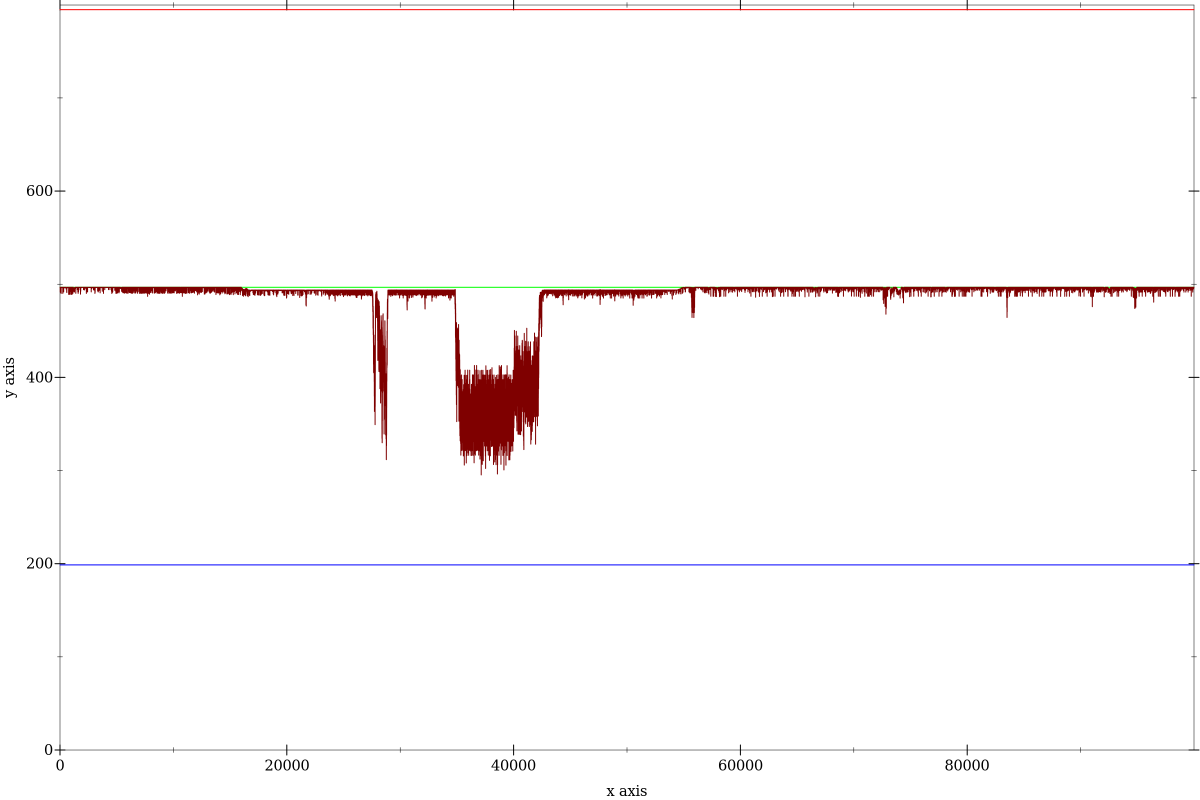
\includegraphics[scale=0.15]{/media/FUN/pd-0118/data690/4pic.png}
\caption{One typical run: $\delta$ = 0.9. a b c d.}
\end{figure}

\section{Players with preference of moderate patience}

\subsection{$\delta$ = 0.8}

\subsubsection{Simulation 5}

I report here a run of 2 000 000 cycles. I would pick some points of interest to investigate further. The first one is the sudden surge from full defection to full cooperation. The second one is when the payoff average drops to half cooperative level. The situation goes worse from there and at some point raises to a moderate level of cooperation again, that would be point 3. After some on and off period, another point of interest would be the one at sudden raise of full cooperation mode. The population is able to maintain that for very long. At some point, it drops and the situation deteriorates.

\begin{figure}[h!]
\center
\includegraphics[scale=0.12]{/home/chi/Downloads/pd-0118/180pic.png}
\includegraphics[scale=0.12]{/home/chi/Downloads/pd-0118/280pic.png}\\
\includegraphics[scale=0.12]{/home/chi/Downloads/pd-0118/380pic.png}
\includegraphics[scale=0.12]{/home/chi/Downloads/pd-0118/480pic.png}
\caption{One typical run: $\delta$ = 0.8 of 2 000 000 cycles.}
\end{figure}

\paragraph{Point 1}
Figure 5.7a , around cycle 500 000, the population suddenly goes up to almost fully cooperative from almost fully defective. The automaton is:

\begin{verbatim}
( .92 .98 .24 .34 .01 ) 
\end{verbatim}

The probability to cooperate in the first round is 0.92 which is very welcoming. The probability to cooperate after a CC is absolute. The probability to cooperate after a betrayal is 0.24 which is punishing. The probability to cooperate after an exploitation is 0.34 which reluctantly continues. The probability to cooperate after a mutual defection is zero. This is tolerating Grim Trigger.

\paragraph{Point 2}
Figure 5.8b, cycle 220 000, there is some evolution. The population is half cooperative but it is a mix of 2 automata:

65\% of this 
\begin{verbatim}
( .74 .83 .02 .17 .05 ) 
\end{verbatim}
and 35\% of this
\begin{verbatim}
( .74 .83 .02 .22 .01 )
\end{verbatim}

These two gives fluctuating payoff sequences. In general the situation is half heartedly cooperative. 

\paragraph{Point 3}
Figure 5.8b, around cycle 450 000, the population is half cooperative. Here is the automaton:

\begin{verbatim}
( .01 .71 .10 .36 .61 )
\end{verbatim}

This automaton starts out defecting. The probability to cooperate after CC and DD is very high. Otherwise low. This is a strange mechanism but the payoff sequence typically is 1 0 4 3 3 3 0 4 4 0 1 1 ... It is a sequence of alternating payoffs, hence averaging at half-heartedly cooperative.

\paragraph{Point 4}

Figure 5.8c, at cycle 300 000, the society is highly cooperative, after that 50 000 cycle, the society goes up to fully cooperative. Here are two automata:

\begin{verbatim}
( .96 .99 .48 .27 .01 )
\end{verbatim}

\begin{verbatim}
( .96 .99 .48 .54 .22 )
\end{verbatim}

At cycle 400 000 and 450 000, there are two automata

\begin{verbatim}
( .97 .99 .59 .11 .62 )
\end{verbatim}

\begin{verbatim}
( .96 .99 .14 .11 .36 )
\end{verbatim}

The population enjoys a long period of full cooperation until the second half of Figure 5.7d.

\subsubsection{Simulation 6}

I report here another run of the same settings.

\begin{figure}[h!]
\includegraphics[scale=0.12]{/media/FUN/pd-0118/data780/1pic.png}
\includegraphics[scale=0.12]{/media/FUN/pd-0118/data780/2pic.png}
\includegraphics[scale=0.11]{/media/FUN/pd-0118/data780/3pic.png}
\caption{One typical run: $\delta$ = 0.8. a b c.}
\end{figure}

\section{Myopic players}

\subsection{$\delta$ = 0.5}

\subsubsection{Simulation 7}
I report here the simulation with individual level of patience dropping to $\delta = 0.5$. It is easy to see that when the individual is impatient, it is hardly possible to keep a cooperative mode for the society. I would only pick the automaton from the rare period of cooperation through out 2 000 000 cycles.

\begin{figure}[h!]
\center
\includegraphics[scale=0.12]{/home/chi/Downloads/pd-0118/150pic.png}
\includegraphics[scale=0.12]{/home/chi/Downloads/pd-0118/250pic.png}\\
\includegraphics[scale=0.12]{/home/chi/Downloads/pd-0118/350pic.png}
\includegraphics[scale=0.12]{/home/chi/Downloads/pd-0118/450pic.png}
\caption{One typical run of 2 000 000 cycles: $\delta$ = 0.5. a b c d.}
\end{figure}

Here is the automaton:
\begin{verbatim}
( .67 .95 .92 .88 .01 ) 
\end{verbatim}

This one is highly tolerant, except for mutual defection. Which means that if people are impatient, it takes extreme virtue to sustain an unstable cooperation. We can see that the situation jumps up then down then up again then deteriorates in a period of 50 000 cycles. The length of this interesting period of activity is around 5\% of the time run. I assume that it would not be necessary to drop the $\delta$ further.

\section{Conclusion}

An one shot game has the gist of an anonymous matching or a match between strangers. In that case, it is natural to behave defectively. On the other hand, a repeated game, in the word of Axelrod, is the situation where there exists informative history and important future. My definition of it is when you have enough data history to form an expectation on how the person would react in a particular situation. Think of people you know, your friends, colleagues etc. In that case where the horizon is lengthened, i.e. there is tomorrow, the cooperation becomes logically possible.\\

In the version of reality I try to approximate here (with probabilistic actions), the players have to be extremely patient (or having long vision) to forge and sustain cooperation. Because the nature of a probabilistic strategy, Defecting as a "mistake" would be something we should learn to expect and the society needs to have some margin of tolerance toward it.\\

Regarding the statement that different degree of patience at individual level paints different patterns for the society at the macro level, I repeat some observations in decreasing order. At a very high level of patience ($\delta = 0.99$) the population spends half the time enjoying a highly cooperative mode. That decreases quickly at $\delta = 0.8$. At $\delta = 0.5$, i.e. a myopic preference, the cooperative period lasts for about 5\%. And in this short 5\% of the time, the virtue of forgiving is extreme.

The second remark is that the society does not swing back and forth between full cooperation and full defection. There exists periods of half-hearted commitments and there are alternate schemes of betrayal and accept being exploited.


\chapter{My proposed approach: the repeated Nash Demand Game}

Since the approach is mostly the same, I only put here the part that is different. The other parts can be found in a previous chapter.

\section{The game}

The Nash Demand Game is the game of dividing a pie. It is a rudimentary example of bargaining behavior. There is a pie of 10 euro to be divided between two players. Each player can make 3 possible claims on the pie: I want a low/ medium/ high portion of the pie. This corresponds to claiming 2 / 5 / 8 euro out of 10. The claims are made simultaneously. If the sum of the claims are compatible (i.e. it is not bigger than the whole 10), each gets what they want. Otherwise, negotiation fails and no one gets anything. Here is the payoff matrix of the game:

\begin{table}[h!]
\center
\begin{tabular}{l|ccc}
\textbf{NDG}&Low& Medium&High\\
\hline
Low & 2,2 & 2,5& *2,8*\\
Medium & 5,2 & *5,5* &0,0\\
High & *8,2*&0,0&0,0\\
\end{tabular}
\caption{Nash Demand Game payoff matrix. The stars mark the Nash equilibria.}
\end{table}

I list some real life examples of the bargaining behavior. It can be the situation between buyer and seller in the market, where they try to divide the distance between the willingness to buy and the willingness to sell. It can be the situation between employer and employee negotiating salary. It can be the situation of claiming natural resources of the earth among conventional nations.\\

The one shot game has 3 pure Nash equilibria (marked in the table) and 1 mixed equilibrium of Low and High strategy. The meaning of this game is that the three pure equilibria are rationally equally viable. It does not matter how the pie is shared, as long as nothing is left or the pie is not wasted, it is considered rationally Pareto. However, the way we see it, there is a perfectly equitable share (which is 5-5) and another type of non-equitable share (which is 8-2 or 2-8). The struggle in the Prisoner's Dilemma is the struggle to achieve a better outcome for the whole society but that outcome is out of Nash's question. (C,C) is not even Nash equilibrium in the first place. Hence the rationale is to try to support that point (C,C) to be stable. Here in the Nash Demand game, all these points are equilibria and they are stable. It is just that there are too many of them and we happen to prefer the equitable share of 5-5 (M-M). That requires both sides to claim modestly immediately and remain that. This simulation is to explore what can really happens in the setting between the one shot and repeated game. Or, in another manner of speaking, to explore how the behavior changes from myopic to patient players.\\

At the end of the simulation result I would solve the game analytically to show how the stability of the 50-50 division is undermined. In brief, switching from the one shot to the repeated setting (i.e. increasing the patience level of the individual in this simulated society) makes the 50-50 division far less stable. The prospect of tomorrow hence the willingness to wait rationalise a new kind of conflict: limited war.\\

\section{Strategy implementation: finite state machine}

Here is an example of a strategy represented by a finite state machine: the one that always cooperates.

\begin{figure}[h!]
\center
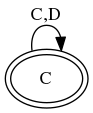
\includegraphics[scale=0.5]{/media/FUN/ndg-0418/dot/C.png}
\caption{The cooperator}
\end{figure}

This machine has one state. The action prescribed in that state is to cooperate. And the arrow with letter C and D means that if the opponent acts C or D in the current round, in the next round this machine stays in the same state of Cooperating. The double circle means that this is the initial state to start with. To illustrate it better, here is the example of another classic strategy: Tit for Tat:

\begin{figure}[h!]
\center
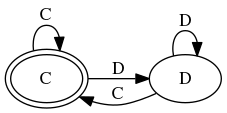
\includegraphics[scale=0.5]{/media/FUN/ndg-0418/dot/T.png}
\caption{Tit for Tat}
\end{figure}

This machine has 2 states. The double circled state which contains letter C is the initial one. Hence this machine starts out cooperating. In the current round if the opponent C, in the next round the machine stays in state C. However if the opponent D, in the next round the machine jumps to state D.

Here is the Grim Trigger:

\begin{figure}[h!]
\center
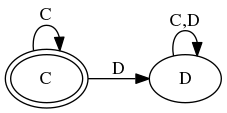
\includegraphics[scale=0.5]{/media/FUN/ndg-0418/dot/G.png}
\caption{Grim Trigger}
\end{figure}

The Grim Trigger starts out by cooperating which is optimistic. As long as the opponent plays C, it stays in the state of Cooperating. Once the opponent switches to D, it jumps to D and never looks back. This one does not forgive and does not forget.\\

The mutation can change initial state, the letter in a circle, the ending point of an arrow or it can add, detach an entire circle.

\subsection{More examples}

Since in this section I run the simulation with the Nash Demand Game, here are some examples of the relevant machines: the one who always claims Low, Medium or High.

\begin{figure}[h!]
\center
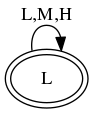
\includegraphics[scale=0.5]{/media/FUN/ndg-0418/dot/L.png}
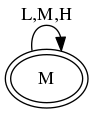
\includegraphics[scale=0.5]{/media/FUN/ndg-0418/dot/M.png}
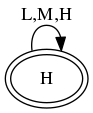
\includegraphics[scale=0.5]{/media/FUN/ndg-0418/dot/H.png}
\caption{Always-low, always-medium, always-high}
\end{figure}

This one is an Accommodator: it starts out playing Medium and chooses what to do next based on how the opponent plays in the previous round. If you play H it retreats to L, if you play M it play M, if you play L it claims H.

\begin{figure}[h!]
\center
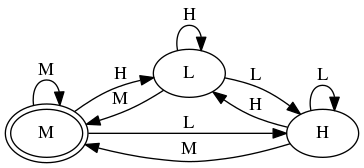
\includegraphics[scale=0.5]{/media/FUN/ndg-0418/dot/A.png}
\caption{Accommodator}
\end{figure}

Here is the payoff sequence of a match between always-low and always-medium:
\begin{table}[h!]
\center
\begin{tabular}{cc|cc}
always-low & always-medium & always-low & always-medium\\
\hline
L & M & 2 & 5 \\
L & M & 2 & 5 \\
L & M & 2 & 5 \\
.. & ..\\
\end{tabular}
\caption{Always-low and always-medium}
\end{table}

between always-medium and always-high:
\begin{table}[h!]
\center
\begin{tabular}{cc|cc}
always-medium & always-high & always-medium & always-high\\
\hline
M & H & 0 & 0 \\
M & H & 0 & 0 \\
M & H & 0 & 0 \\
.. & ..\\
\end{tabular}
\caption{Always-medium and always-high}
\end{table}


To get a glimpse of the Accommodator character, let's match it with the always-low, always-medium, always-high and itself:

\begin{table}[h!]
\center
\begin{tabular}{cc|cc}
always-low & accommodator & always-low & accommodator\\
\hline
L & M & 2 & 5 \\
L & H & 2 & 8 \\
L & H & 2 & 8 \\
.. & ..\\
\end{tabular}
\caption{Always-low and accommodator}
\end{table}

\begin{table}[h!]
\center
\begin{tabular}{cc|cc}
always-medium & accommodator & & \\
\hline
M & M & 5 & 5 \\
M & M & 5 & 5 \\
M & M & 5 & 5 \\
.. & ..\\
\end{tabular}
\caption{Always-medium and accommodator}
\end{table}

\begin{table}[h!]
\center
\begin{tabular}{cc|cc}
always-high & accommodator &  & \\
\hline
H & M & 0 & 0 \\
H & L & 8 & 2 \\
H & L & 8 & 2 \\
.. & ..\\
\end{tabular}
\caption{Always-high and accommodator}
\end{table}

\begin{table}[h!]
\center
\begin{tabular}{cc|cc}
accommodator & accommodator &  & \\
\hline
M & M & 5 & 5 \\
M & M & 5 & 5 \\
M & M & 5 & 5 \\
.. & ..\\
\end{tabular}
\caption{Accommodator and itself}
\end{table}

We can see that, in the match with always-low, the accommodator switches to play High from the second round. In the match with always-high, the accommodator switches to play Low from the second round. These are not to waste the resources.

\section{How to interpret the result}

By representing strategies in finite state machines, how we read the result becomes qualitatively different from using a Markov structure. When the number of states of the machine is small, it is easier to lay out its scheme and describe it in a comprehensible and sensible way. When the number of states is really big, the contingency becomes huge hence the plan even if laid out becomes unnecessarily incomprehensible. It would make better sense to look at what the machine does in action instead of looking at its algorithm. Which means that we would look at its payoff sequence resulting from matching with classic machines. In other words, we would look at how it interacts with a benchmark set of classic machines. The intuition is that if we cannot tell who you are, we watch your interaction with other known members and we make deduction on your revealed nature.\\

The benchmark is the set of classic machines that the simple character has already been established. They are the always-lows, always-medium, always-high and the accommodator.\\

Taking the number of rounds to be 500, and the $\delta$ to be 0.99. 

\begin{table}[h!]
\center
\begin{tabular}{l|cccc}
\textbf{0.99}& always-low & always-medium & always-high & accommodator\\
\hline
always-low    & 199 199 & 199 497 & *199 795*  & 199 792 \\
always-medium & 497 199 & *497 497* & 0 0      & 497 497 \\
always-high   & *795 199* & 0 0     & 0 0      & 787 197 \\
accommodator  & 792 199 & 497 497 & 197 787  & 497 497 \\
\end{tabular}
\caption{Payoff benchmark, and equilibria}
\end{table}

There are 3 pure Nash equilibria which are marked with stars in the table. Now if we add a random machine into this benchmark matrix, it may or may not change the status quo of the equilibrium points. Let's take an example that shakes up the status quo:
\begin{table}[h!]
\center
\begin{tabular}{l|ccccc}
\textbf{0.99}& machine a & always-low & always-medium & always-high & accommodator\\
\hline
machine a & *322.9 322.9* &  670.8 198.7  &  267.7 267.7  &  80.6 322.5   &  532.5 297.2  \\
always-low &   198.7 670.8  &  198.7 198.7  &  198.7 496.7 &  *198.7 794.7* &  198.7 791.7  \\
always-medium  &  267.7 267.7  &  496.7 198.7 &  *496.7 496.7*   &    0 0   &     496.7 496.7* \\
always-high &  322.5 80.6  &  *794.7 198.7*  &     0 0   &         0 0      & *786.7 196.7  \\
accommodator  &  297.2 532.5  &  791.7 198.7 &  *496.7 496.7  &  196.7 786.7* &  496.7 496.7  \\
\end{tabular}
\caption{The stability of a random strategy}
\end{table}

In this table, we can see that machine a forms an equilibrium with itself. And in this equilibrium, the payoff average (which is 322.9) is less than the case of an always-medium equilibrium (which is 496.7). This is a strategy that sustain wasteful negotiation in the society. It is able to form a stable equilibrium with itself usually because it is able to resist always-high. If it submits to always-high or accommodator, the star would go to the always-high or accommodator. In other word, always-high or accommodator would be a better response to this strategy than it is to itself.\\

\subsection{Evolutionarily stable strategy}

The central concept in evolutionary game theory is about an evolutionarily stable strategy, proposed by Maynard Smith \cite{maynard}. This concept is used to describe the persistence of one strategy against another strategy, illuminating in a population context. The scenario is as following: there is one population hosting exclusively strategy A. A can be a pure or a mixed strategy. When there is $\epsilon$ mutation B entering the population, A is said to be evolutionarily stable against B if A can repel B. In the other way around, B invades the population of A. On the middle ground, they are neutrally stable which means that they coexist at any possible ratios.

For example, in the one shot prisoner's dilemma, there are only two strategies: to play C and to play D. Let's say there is a population of people playing D, hence strategy D is an incumbent. By mistake, some people switch to play C, hence strategy C is a mutant.

\begin{table}[h!]
\center
\begin{tabular}{l|ccccc}
\textbf{PD}& C & D \\
\hline
C & 3 &  0   \\
D &  4  & 1   \\
\end{tabular}
\caption{In the one shot prisoner's dilemma, D is evolutionarily stable against C}
\end{table}

To answer the question, whether D is evolutionarily stable against mutant C, we consider two criteria:

- First, when being matched with the incumbent D, an incumbent D gets 1 while a mutant C gets 0. $1 > 0$ hence the weakest definition of rationality prescribes to prefer D.

- Second, when being matched with the mutant C, an incumbent D gets 4 while a mutant C gets 3. $4 > 3$ hence the incumbent D is still doing better.

The incumbent is doing better than the mutant in both cases: matched with the incumbent and matched with the mutant. Hence the mutant is unable to spread in the population and the incumbent is stable.


Consider the example in the repeated Nash Demand game:

\begin{table}[h!]
\center
\begin{tabular}{l|ccccc}
\textbf{0.99}& machine a & always-medium \\
\hline
machine a & *322.9 322.9* &   267.7 267.7   \\
always-medium  &  267.7 267.7  &    *496.7 496.7*  \\
\end{tabular}
\caption{Machine a is stable against always-medium.}
\end{table}

The stars indicate two pure Nash equilibria. However, in the context of evolutionarily stable concept, to answer the question, whether the incumbent a is stable against the invasion of the mutant always-medium, we consider two criteria:

- First, when being matched with the incumbent a, a machine a gets 323 while a mutant always-medium gets 268. $323 > 268$ hence the incumbent is already doing better than the mutant. The mutant cannot spread. We do not need the second criteria because the incumbent is already the best response to itself.

- Second, when being matched with the mutant always-medium, a machine a gets 268 and a mutant always-medium gets 497. $268 < 497$ this is to say that the mutant is also a best response to itself and it would be stable against this machine a if it is the incumbent.

In the case above machine a is able to resist the invasion of always-medium because machine a is not kind to always-medium. It gives always-medium not enough point. Let's consider another example where machine a gives always-medium enough point to destabilise itself:

\begin{table}[h!]
\center
\begin{tabular}{l|ccccc}
\textbf{0.99}& machine a & always-medium \\
\hline
machine a & 322.9 322.9 &   267.7 400*   \\
always-medium  &  *400 267.7  &    *496.7 496.7*  \\
\end{tabular}
\caption{Example continued: machine a is no longer stable.}
\end{table}

When being matched with the incumbent a, a machine a gets 323 while a mutant always-medium gets 400. $323 < 400$ hence always-medium would easily take over the population. Machine a is no longer a best response to itself because it gives too much payoff to the mutant always-medium. Machine a is no longer a Nash equilibrium, it has lost all the stars.

\begin{table}[h!]
\center
\begin{tabular}{l|ccccc}
\textbf{0.99}& machine a & always-medium \\
\hline
machine a & *322.9 322.9* &   267.7 322.9*   \\
always-medium  &  *322.9 267.7  &    *496.7 496.7*  \\
\end{tabular}
\caption{Example continued: machine a is not evolutionarily stable.}
\end{table}

In this case, when being matched with the incumbent, an incumbent a gets 322.9 and a mutant always-medium gets the same point 322.9. So they are equally fit. Here is where we should consider the second criterion: when being matched with the mutant, an incumbent a gets 267.7 while a mutant always-medium gets 496.7. The mutant is able to get better for themselves and the mutant does not treat the outsider kindly. Hence in this case machine a is not an ESS, even though it is still a Nash equilibrium of the game. The evolutionarily stable concept is then considered a stringent (refinement) of the Nash equilibrium concept.

If they get equal payoff everywhere they are neutrally stable and they can coexist at any possible rate. The population can drift between the two for decades.

That's for the evolutionarily stable concept for the interpretation of my simulation result. Another important remark is that the game has changed from 2x2 to 3x3. This change makes the strategies become so much more complex and so much more dimensional. An example is that one machine can have 100 states and this 100 states can generate explosive numbers of contingency. It is impossible to interpret all these contingencies in a comprehensible manner. I have given up on imposing a scheme of personality test to evaluate the characteristic of the all strategies. I use certain indications but I remain to proceed case by case.\\

\chapter{Simulation result: the repeated Nash Demand Game}
\section{Patient players}

I run with the following configurations: the population has a fixed N agents and N = 100. The number of rounds to be played when two agents are matched is 500. The delta to calculate present value of the 500 payoff sequence is 0.99. The learning rate is 10 percent. The mutation rate is 2 percent.

$\delta = 0.99$ is very close to 1. This represents a highly patient agent. Then I plot the average payoff of the whole population, with 3 benchmarks. The red line is the hypothetical payoff resulting from a sequence of highest possible payoff: 8. The blue line is the hypothetical payoff resulting from a sequence of all payoffs of 2. The green line is when there is 5 everywhere (i.e. everyone is claiming 5 all the time). I increase the mutation rate because the strategy space of a 3x3 game is exponentially bigger than the strategy space of a 2x2 game.\\

\subsection{$\delta = 0.9$}

\subsubsection{Simulation 1}

\begin{figure}[h!]
\center
\includegraphics[scale=0.2]{/home/chi/Downloads/ndg-0418-3/991pic.png}
\caption{One typical run of 1 000 000 cycles: $\delta$ = 0.99}
\end{figure}

Overall I would like to make some brief comments. The first one is that the population is constantly in non-equitable sharing state. There is very little time that the 50-50 division holds. The second one is that in these periods where the population average payoff is less than ideal but not very low. Most of that is due to strategies that waste resources in a period of sustained conflict in the length of several rounds. The probing behavior is not necessarily in the initial period. It can happen after that for a while. Which makes the population average to be less than ideal but not less very much. This kind of strategy is fair but only after a show of strength, some probing and some retaliation. The third one is that there are periods that the population average is extremely low and chaotic. This one is due to a mixture of truly aggressive strategy and its submission (aggressor and accommodator). This one can legitimately be a stable mixture. Lastly, there are periods that the population average is not perfect but it can be due to a bad luck in mutation or it is an unstable state waiting for the right mutation to appear.\\

For further information, I plot the first 50K cycle of Figure 7.1. This short period includes the stable 50-50 division, its collapse and raise up again. Hence we would be able to watch in action the series of events leading to its fall and see in details what helps to pave its way back. It comes back less than ideal a little (due to an initial period of probing), but would be back to full 50-50 division at around cycle 200000.

\begin{figure}[h!]
\center
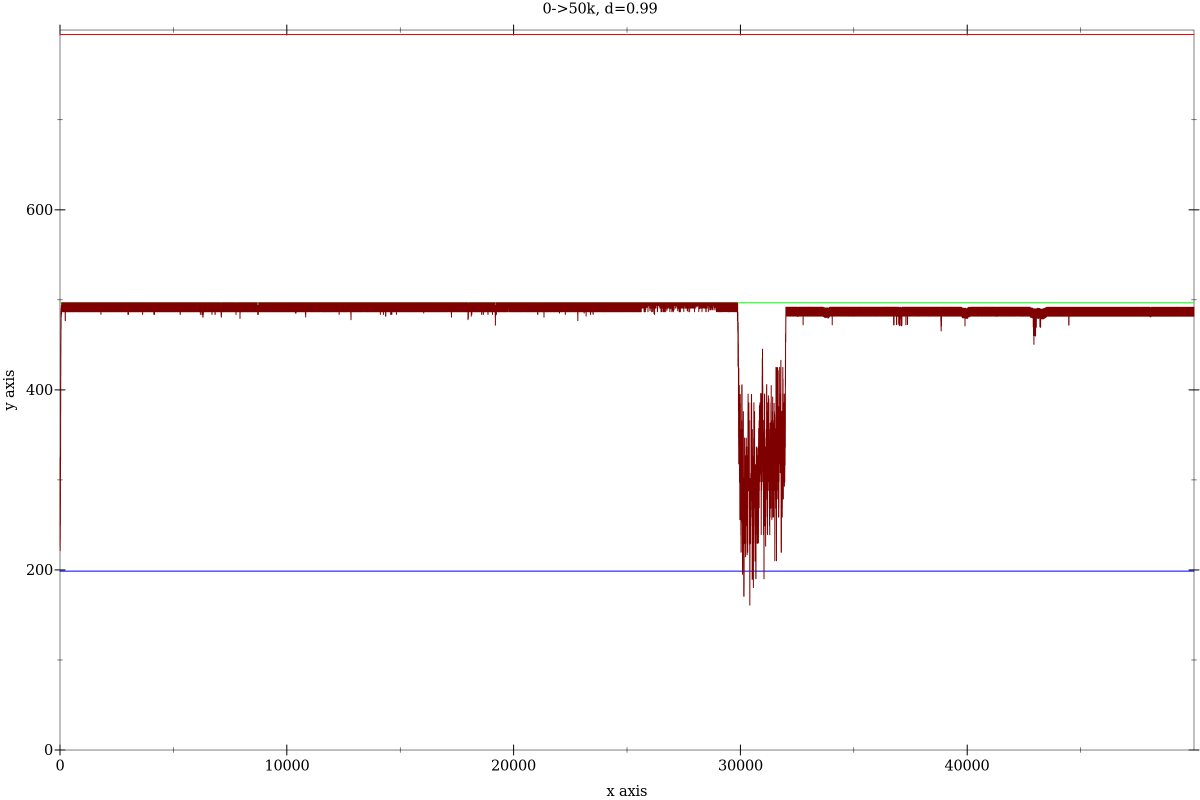
\includegraphics[scale=0.2]{/media/FUN/ndg-0418/99150k.png}
\caption{$\delta$ = 0.99, cycle 1 -> 50K}
\end{figure}

\paragraph{Point 1}

Until cycle 25000 (or precisely cycle 24800), the population is full of all-medium strategies. The description of an always-medium strategy is that it plays fair to itself, to always-low, to the accommodator and it gives always-high zero payoff. Because it gives always-high nothing, it is able to resist always-high invasion.

\begin{figure}[h!]
\center
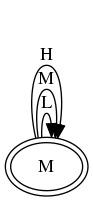
\includegraphics[scale=0.5]{/media/FUN/ndg-0418/dot99/25k.png}
\caption{all-medium strategy, at cycle 25K}
\end{figure}

\begin{table}[h!]
\center
\begin{tabular}{l|ccccc}
\textbf{0.99}& always-low & always-medium & always-high & accommodator\\
\hline
always-medium  &  496.7 198.7 &  *496.7 496.7*   &    0 0   &     496.7 496.7* \\
\end{tabular}
\caption{From cycle 0 to cycle 24800: always medium}
\end{table}

We would see the evolution of the strategy from cycle 24800 to cycle 30K which is the transition from perfectly equitable strategy to a chaotic collapse.\\

From cycle 24800 to cycle 25800, the strategy is no longer the always-medium because it has mutated a new feature: it gradually submits to always-high strategy. The always-medium strategy is always fair with itself, with the always-low and the accommodator. And it resists the always-high completely, i.e. it does not gives always-high a single point because it never submits to the aggressive claim of always-high. It insists on claiming 5 while always-high insists on claiming 8. Because of this, always-medium is a best response to itself. It is able to form an equilibrium with itself. From cycle 24800 to cycle 25800, the machine starts to submit to always-high, i.e. it claims 2 and always-high starts to get a lot of points. The behaviors with other classic strategies do not change yet, for example, it still claim 5 toward itself, always-low, and accommodator. But it starts to submit if the opponent claims aggressively. In this period, the always-medium equilibrium is still stable because the point it gives to always-high is not high enough. Always-high is still not a best response and it is still a best response to itself. This situation changes quickly.

\begin{table}[h!]
\center
\begin{tabular}{l|ccccc}
\textbf{0.99}& always-low & always-medium & always-high & accommodator\\
\hline
the compromised always-medium  &  496.7 198.7 &  *496.7 496.7*   &    57 228   &     496.7 496.7* \\
\end{tabular}
\caption{From 24800 to 25800, cycle 25100: always-medium is compromising toward always-high. Not enough to destabilise itself, but soon.}
\end{table}



\paragraph{Point 2}


At cycle 25900, the machine is no longer a stable equilibrium. It has gives always-high enough point to destabilise the 50-50 division. Always-high has become a best response to the current strategy of the population.

\begin{table}[h!]
\center
\begin{tabular}{l|ccccc}
\textbf{0.99}& always-low & always-medium & always-high & accommodator\\
\hline
the compromised always-medium  &  496.7 198.7 &   496.7 496.7   &    175 700*   &     496.7 496.7 \\
\end{tabular}
\caption{Cycle 25900: the compromised strategy. It can no longer be called an always-medium, even though it still plays fair with itself, always-low, and accommodator.}
\end{table}


\begin{figure}[h!]
\center
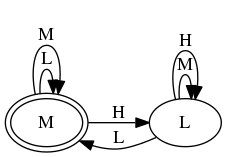
\includegraphics[scale=0.5]{/media/FUN/ndg-0418/dot99/26k.png}
\caption{At cycle 26K, the strategy evolves to accommodate aggressive opponent. But the situation is still fine because no one happens to be aggressive yet. It is a Compromised strategy. On face value, it happens to generate fairness exactly as it is supposed to do, but it has a branch that reaches out to all-high invasion.}
\end{figure}

The reason is that since 25900, the machine mutates another state with a new contingency (which is a security breach): if the opponent plays High, it switches to the newly added state of playing Low instead of insisting on playing Medium. This happens off equilibrium path. It goes silent because in the society people keep claiming Medium to each other and the population payoff average is still ideal all the time. No one happens to claim High in this environment hence no one ever knows that the other would retreat immediately.

Here I make a less relevant remark. Binmore makes a fortified concept of the ESS: the modified evolutionarily stable strategy. It is due to the idea in Rubinstein's paper that: in a fortified equilibrium, the machine drops the unnecessarily state. Hence the machine in figure 7.4 would not be considered a MESS because it has a state of playing Low that is never reached in the equilibrium scenario of the 50-50 division.

Anyway, back to my simulation. From this point on, the strategy opens itself to the possibility of submitting to aggressive negotiator, however, it does not itself consider that possibility yet. As I show in the table later, it does not learn to exploit the Accommodator or the always-low, one that submits immediately if you go bold.

Overall in this period, the population average payoff is still fully equitable. Everybody is still sharing 50-50 all the time. But the sustaining mechanism is not the same as the always-medium. The difference is that always-medium is able to resists always-high. This strategy a is fair to itself all the time but it submits to always-high. It plays low all the time in response to always-high. This one is neutral to always-medium and by some random drift its percentage in the population grows up very fast.

This neutral mutant makes the population weak because it is vulnerable to all-high strategy. It submits completely to always-high hence it is unable to maintain an equilibrium with itself. It is unstable. As I show in the table, it still generates equitable shares among itself but the fact that it submits to all-high makes it no longer best response to itself. all-high becomes the best response to this machine. It is just that in this situation, everybody is claiming Medium all the time and no one happens to discover that they can play aggressively all the time yet.

\begin{table}[h!]
\center
\begin{tabular}{l|ccccc}
\textbf{0.99}& machine a & always-low & always-medium & always-high & accommodator\\
\hline
machine a & 496.7 496.7  &  496.7 198.7  & *496.7 496.7  &  196.7 786.7* &  496.7 496.7  \\
always-low  &  198.7 496.7  &  198.7 198.7  &  198.7 496.7 &  *198.7 794.7* &  198.7 791.7  \\
always-medium   & 496.7 496.7*  & 496.7 198.7 &  *496.7 496.7*  &     0 0   &     496.7 496.7* \\
always-high   &*786.7 196.7  & *794.7 198.7*   &    0 0     &       0 0   &    *786.7 196.7  \\
accommodator   & 496.7 496.7 &   791.7 198.7 &  *496.7 496.7  &  196.7 786.7*  & 496.7 496.7 \\
\end{tabular}
\caption{Machine a at cycle 26k. It no longer is a best response to itself, which is a security breach, because it opens to the possibility of accommodating aggressive claims. It does not contemplate itself on playing aggressive though.}
\end{table}


\paragraph{Point 3}

\begin{figure}[h!]
\center
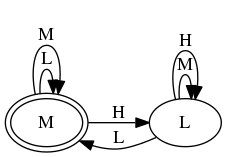
\includegraphics[scale=0.5]{/media/FUN/ndg-0418/dot99/27k1.png}
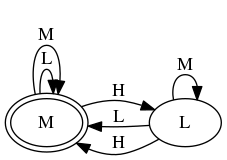
\includegraphics[scale=0.5]{/media/FUN/ndg-0418/dot99/27k2.png}
\caption{At cycle 27K, 85\% machine a submitting to all-high completely and 15\% machine b submitting to all-high half the time.}
\end{figure}

In cycle 27K, the mutated machine b actually can handle all-high strategy. It submits to all-high only half the time hence able to resist the invasion of all-high strategy.

\begin{table}[h!]
\center
\begin{tabular}{l|ccccc}
\textbf{0.99}& machine b & always-low & always-medium & always-high & accommodator\\
\hline

machine b & *496.7 496.7*  &  496.7 198.7  & *496.7 496.7  &  99 395 &  496.7 496.7  \\
always-low  &  198.7 496.7  &  198.7 198.7  &  198.7 496.7 &  *198.7 794.7* &  198.7 791.7  \\
always-medium   & 496.7 496.7*  & 496.7 198.7 &  *496.7 496.7*  &     0 0   &     496.7 496.7* \\
always-high   & 395 99  & *794.7 198.7*   &    0 0     &       0 0   &    *786.7 196.7  \\
accommodator   & 496.7 496.7 &   791.7 198.7 &  *496.7 496.7  &  196.7 786.7*  & 496.7 496.7 \\

\end{tabular}
\caption{Machine b at cycle 27k. It is best response to itself and has all the stars. This one is an always-medium strategy. The compromise is not serious yet. It is still able to resist always-high. Machine a, on the other hand, cannot.}
\end{table}

If machine b can grow up in numbers, the population can be stable again, the security breach is closed. However, because there is no force to push against machine a or machine b, the percentages of them are just due to random drift. They both get the same payoffs, they play fair among themselves and to each other. They coexist peacefully together. It is just that behind the facade, one is secretly compromised, one is not.

At cycle 28k and cyle 29k, fate takes a turn and the evolution drifts toward the weak one. The strategies become vulnerable to all-high.

\paragraph{Point 4}

At cycle 30000, the 50-50 division norm collapses. The population is a mixture of 3 machines.

\begin{figure}[h!]
\center
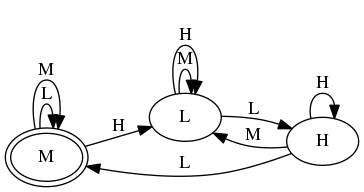
\includegraphics[scale=0.5]{/media/FUN/ndg-0418/dot99/30k1.png}
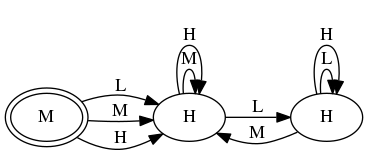
\includegraphics[scale=0.5]{/media/FUN/ndg-0418/dot99/30k2.png}
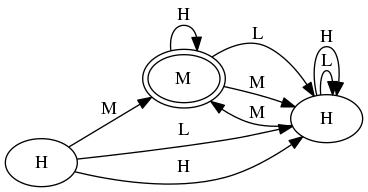
\includegraphics[scale=0.5]{/media/FUN/ndg-0418/dot99/30k3.png}
\caption{At cycle 30K, 41\% machine c, 34\% machine d, 25\% machine e.}
\end{figure}

I would describe here the machine and the payoff sequence they get. \\

Machine c is very fair to itself, but it submits quickly to machine d and machine e. This explains the chaos in the population payoff average. There are two sequences of 5s (5 5 5 5...) for the match of machine c with itself. But there would be a sequence of 2s (2 2 2 2...) and a sequence of 8s (8 8 8 8...) for the match between machine c and machine d or e. The match between machine d and e creates two sequences of 0s (0 0 0 0...) because they do not claim compatible shares.

If you have a look at machine c, you would see that it starts by playing Medium. If opponent plays High it plays Low, and it is able to switch to play High if opponent plays Low. This machine has evolved to be able to exploit. The previous ones learn to submit to all-high but this one has gone one step further, it has learned to be flexible enough and play aggressive. It has a touch of an Accommodator.

Please have a look at machine d, it plays Medium for only the first round. Then it has two extra states but both claiming High. This one is almost the all-high strategy.

Machine e also looks complicated but it has only 2 states. There is a redundant state that there is no way to reach it from anywhere inside the machine.

Because machine d and e does not have a state of playing Low, they play it aggressively to each other all the time, they both get 0 if being matched. Machine c is to cushion the aggression because it has a state of playing Low.

Overall, we should treat this mixture as one. This mixture is hostile toward always-high because it has enough aggressive machines in its mix. It also learns to exploit always-low and accommodator. The best response to this kind of strategy is the accommodator. This kind of situation (a mixture between aggressor and accommodator) happens from 29900 to 31900.


\begin{table}[h!]
\center
\begin{tabular}{l|ccccc}
\textbf{0.99}& mixture 1 & always-low & always-medium & always-high & accommodator\\
\hline

mixture 1 & *322.9 322.9* &  670.8 198.7  &  267.7 267.7 &   80.6 322.5 &     532.5 297.2 \\
always-low  &  199 671  &  198.7 198.7  &  198.7 496.7 &  *198.7 794.7* &  198.7 791.7  \\
always-medium   & 268 268  & 496.7 198.7 &  *496.7 496.7*  &     0 0   &     496.7 496.7* \\
always-high   & 322 87  & *794.7 198.7*   &    0 0     &       0 0   &    *786.7 196.7  \\
accommodator   & 297 532 &   791.7 198.7 &  *496.7 496.7  &  196.7 786.7*  & 496.7 496.7 \\

\end{tabular}
\caption{The mixture at cycle 30k. So much resource wasted because of the match between aggressive claimaints. Note that this mixture has become slightly aggressive to always-low and the Accommodator.}
\end{table}

\paragraph{Point 5}

At cycle 31K, the mixture evolves better: 58\% machine e and 42\% machine f. Machine e is an all-high machine. Machine f is almost an accommodator, it is flexible.

This explains why they maintain the mixture of half each. Machine f submits to machine e. Machine f is fair with itself. Machine e is zero with itself.

\begin{figure}[h!]
\center
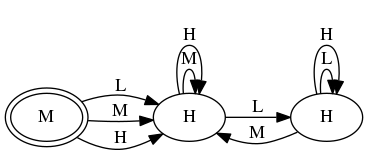
\includegraphics[scale=0.5]{/media/FUN/ndg-0418/dot99/31k1.png}
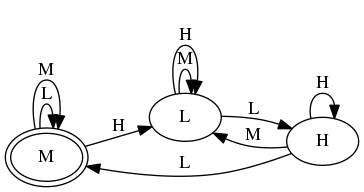
\includegraphics[scale=0.5]{/media/FUN/ndg-0418/dot99/31k2.png}
\caption{At cycle 31K, 58\% machine e, 42\% machine f.}
\end{figure}

If you look at the character of machine e, it only has a state of playing High. It is an all-high strategy. Machine f has 3 states of Low, Medium and High. This mixture is not overall stable though. The population average quickly raises up after 1000 cycle.\\


\begin{table}[h!]
\center
\begin{tabular}{l|ccccc}
\textbf{0.99}& mixture 2 & always-low & always-medium & always-high & accommodator\\
\hline

mixture 2 & 328.9 328.9  &  667.8 198.7  &  211.5 211.5  &  82.6 330.4* &    663.2 324.4 \\
always-low  &  199 678  &  198.7 198.7  &  198.7 496.7 &  *198.7 794.7* &  198.7 791.7  \\
always-medium   & 212 212  & 496.7 198.7 &  *496.7 496.7*  &     0 0   &     496.7 496.7* \\
always-high   & *330 83  & *794.7 198.7*   &    0 0     &       0 0   &    *786.7 196.7  \\
accommodator   & 324 663 &   791.7 198.7 &  *496.7 496.7  &  196.7 786.7*  & 496.7 496.7 \\

\end{tabular}
\caption{The mixture at cycle 31k. It is no longer stable because it gives always-high more than it gives to its own kind.}
\end{table}

\paragraph{Point 6}

At 31900, there appears a new pure strategy that is able to be stable. It takes over the stable mixture of aggressor and accommodator. It shares certain features with the mixture: it exploits the weaks (always-low and accommodator) and it resists the aggressors (always-high), it resists the always-medium. But most importantly, the sufficient condition is that it is fair enough among itself when it recognises itself hence it is able to form an equilibrium with itself. This is a remarkable strategy. It is a tough strategy.

\begin{table}[h!]
\center
\begin{tabular}{l|ccccc}
\textbf{0.99}& tough & always-low & always-medium & always-high & accommodator\\
\hline
tough & 492 492* & 792 199  &  5 5  & 0 0  &  784 200  \\
\end{tabular}
\caption{Starting at 32100, a tough kind.}
\end{table}

From 32000, the population payoff average comes right back to the ideal level, a little less. The strategy is to resist always-high completely and be kind enough to its own kind. This machine recognises its own kind by probing in the first round. The payoff sequence hence 0 5 5 5 5 ... It plays aggressively in the first round but then retreat to play Medium onwards. It does not retreat with always-high. It does not be kind to always-Medium. It even recognises to exploit always-low and accommodator. I think that this one is a remarkable strategy. It has the ability to recognise one's own kind to play it fair with itself. It repels always-high, always-medium and exploits always-low and forces accommodator to submit to it. 

The accommodator would be able to play fair with itself, exploit all-low, submit to all-high. This one, with an extra state, is able to distinguish between an accommodator and its own kind. It exploits accommodator while still be kind to itself. Plus, it resists always-high and always-medium. It forms an equilibrium with itself in the presence of all formidable strategies. It is a tough player.

\begin{table}[h!]
\center
\begin{tabular}{l|ccccc}
\textbf{0.99}& tough & always-low & always-medium & always-high & accommodator\\
\hline

tough & *491.8 491.8*  & 791.7 198.7  &      5 5    &        0 0 &       783.8 199.7  \\
always-low  &  198.7 791.7  &  198.7 198.7  &  198.7 496.7  & *198.7 794.7*  & 198.7 791.7  \\
always-medium  &      5 5 &        496.7 198.7   &*496.7 496.7*&       0 0 &       496.7 496.7* \\
always-high  &      0 0    &   *794.7 198.7*     &  0 0   &        0 0    &   *786.7 196.7  \\
accommodator  &  199.7 783.8  &  791.7 198.7  & *496.7 496.7    &196.7 786.7*  & 496.7 496.7 \\
  \end{tabular}
\caption{Cycle 32100 The tough strategy matching with others}
\end{table}


\begin{figure}[h!]
\center
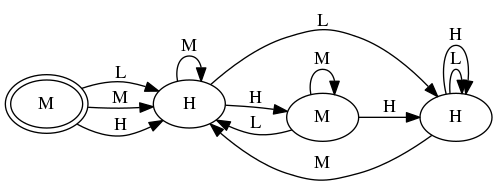
\includegraphics[scale=0.5]{/media/FUN/ndg-0418/dot99/32k.png}
\caption{At cycle 32000, a tough negotiator. Tough 1}
\end{figure}

Actually, at cycle 32000, the percentage of this machine is 95\% and it raises to 100\% quickly after that.

The situation is stable until cycle 43000 where appears another mechanism. It is another kind of tough strategy, though. It probes in the second round hence the payoff sequence 5 0 5 5 5 5... It is able to distinguish the previous kind of tough with itself, hence it gives itself 492 point while it gives the previous tough machine less, 486. Funny thing is that the previous tough would give itself 492 but gives this one 486. They both use the initial rounds to probe and recognise themselves. This is the defining feature of a tough machine.

\begin{table}[h!]
\center
\begin{tabular}{l|ccccc}
\textbf{0.99}& tough & always-low & always-medium & always-high & accommodator\\
\hline
tough & 492 492* & 795 199  &  0 0  & 0 0  &  786 197  \\
\end{tabular}
\caption{At 43500, another tough kind.}
\end{table}
\begin{figure}[h!]
\center
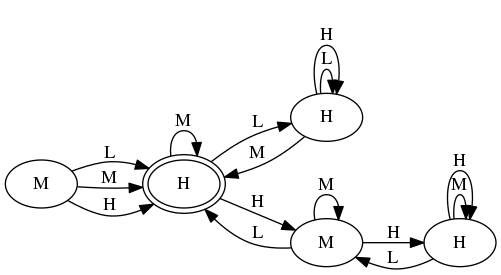
\includegraphics[scale=0.5]{/media/FUN/ndg-0418/dot99/99143500.png}
\caption{At cycle 43500, another tough negotiator. Tough 2}
\end{figure}

This kind of tough machine takes reign for an incredibly long period, until cycle 99800. Where a mutation happens that starts to reach out to always-medium. From cycle 99800 to 100800, the mutation gives always-medium some point though not enough to destabilise the status quo. At the same time of 100800, another mutation takes place that starts to submit to always-high and exploits accommodator and always-low less. The mutation is make the strategy less aggressive. It starts to play fair with itself, the always-medium, and the accommodator. It plays Low with always-low and gives always-high some more point. All these mutations happening but it is still stable because it still resists always-high. It can be said to be some kind of always-medium.

From 106000 to 117100, the strategy is almost always-medium and still stable, but it grows to exploits always-low. After that, the mutation goes away silently. The strategy is to play fair with itself, always-medium, accommodator. It plays low with always-low and gives always-high some point. From 123900, it gives always-high 0 and is not kind to accommodator but the stability remains. From 138400, it starts to give always-high some point again.

From 147900, the population is a mixture of two machines. One machine (84\%) submits to the accommodator completely and the accommodator becomes the best response. It still plays fair to itself and the always-medium. It plays Low to always-low and gives always-high some point. But it gives the accommodator a whole lot of points and it is no longer stable. The other machine (16\%) is still able to form an equilibrium with itself. However, overall, as a mixture, the population submits to accommodator and is not stable.

\begin{table}[h!]
\center
\begin{tabular}{l|ccccc}
\textbf{0.99}& x & always-low & always-medium & always-high & accommodator\\
\hline

x & 492 492 & 205 199  &  492 492  & 65 260  &  199 707*  \\
\end{tabular}
\caption{At 147900, this mixture submits to the accommodator.}
\end{table}

This situation goes on until cycle 177000 where a new machine learns to play fair with itself, and the accommodator hence reducing the dominating point of the accommodator. It does not play fair completely with itself hence the always-medium machine becomes stable. But this one persists unstably for very long time, waiting for the always-medium to happen.

\begin{table}[h!]
\center
\begin{tabular}{l|ccccc}
\textbf{0.99}& x & always-low & always-medium & always-high & accommodator\\
\hline

x & 494 494 & 356 199  &  491 496*  & 0 0  &  476 486  \\
\end{tabular}
\caption{At 177000, this machine keeps the accommodator at bay.}
\end{table}

At cycle 225500, the always-medium actually happens. It plays fair with itself, the always-medium, always-low and accommodator. It gives little point to always-high. As you can see on the population average graph, this is the only other period in which the population payoff average reaches absolute level of fairness - where true 50-50 division holds, where everybody simply claims 5 from the first round onward, no sustained conflict (i.e. no war) because of no probing, no retaliation, no waste of resources.

\begin{table}[h!]
\center
\begin{tabular}{l|ccccc}
\textbf{0.99}& x & always-low & always-medium & always-high & accommodator\\
\hline

x & 497 497* & 497 199  &  497 497*  & 30 122  &  497 497*  \\
\end{tabular}
\caption{At 225500, the always-medium actually happens and it happens for some time.}
\end{table}

At 270400, some bad luck just happens in the mutation hence the population payoff average reduces. At around 278400, a new mixture becomes stable, it does badly with everything else but good enough with itself. It gradually becomes fair with always-low and always-medium, not enough to destablise itself. It grows to be fair with accommodator also.

From 343100 to 350700, the machine is vulnerable toward a tough machine but a tough machine never emerges so it sustains its stability. In general, this one keeps the aggressive types at bay. It becomes less kind with always-medium also.

At 494800, it grows kind enough to always-medium for always-medium to take over but always-medium does not appear. It is vulnerable to the invasion of always-medium till 898000. 
\begin{table}[h!]
\center
\begin{tabular}{l|cccccccc}
\textbf{0.99}& x & always-low & always-medium & always-high & accommodator &tough 1 & tough 2\\
\hline
x& 470.5 470.5* &424.1 198.7&  246.0 246.0 &  95.0 380.1 & 231.1 326.5&   94.1 376.2 &  94.9 379.7\\  
\end{tabular}
\caption{At 898000, a complicated tough negotiator.}
\end{table}
This strategy does badly with everything else. It takes a prolonged period to probe and apologise and probe again to distinguish its own kind. The payoff is 470 because the sequence is 0 0 2 2 2 5 2 0 5 5 5 5 5 5... Eventually they settle down and claim 5 onward.

At 915000, there is a transition to another machine that is vulnerable to the invasion of always-medium.
\begin{table}[h!]
\center
\begin{tabular}{l|cccccccc}
\textbf{0.99}& x & always-low & always-medium & always-high & accommodator &tough 1 & tough 2\\
\hline
x& 479.0 479.0 & 230.7 198.7 & 342.0 491.7*  &96.9 387.6&  294.8 258.6&   96.9 387.6&  100.8 400.2\\ 
\end{tabular}
\caption{At 915000, a window opens for the invasion of always-medium.}
\end{table}
At 937500, the window for always-medium closes and another mutation opens a window for always-high to appear. If always-high appears it would definitely drops the population payoff average. However always-high does not appear till the end of the simulation.
\begin{table}[h!]
\center
\begin{tabular}{l|cccccccc}
\textbf{0.99}& x & always-low & always-medium & always-high & accommodator &tough 1 & tough 2\\
\hline
x& 479.0 479.0&  263.9 198.7&  342.0 491.7&  192.8 771.1*& 250.4 198.3 & 192.8 771.1*& 100.8 400.2 \\
\end{tabular}
\caption{At 937500, a window opens for the invasion of always-high.}
\end{table}

\section{Characteristic evaluation and interpretation}

At this point, I would like to develop a systematic characteristic test. I would try to identify the accommodator, the tough negotiator, the always-medium, and always-high. Also the one that on the face value is fair with itself and fair with always-medium hence it coexists peacefully in the population. But this one is weak and unable to resist invasion. It submits to always-high. It is a compromised strategy.\\

So the story goes that always-high never learns to share equitably with its own kind, but one that learns to do so would have the sufficient condition to form an equilibrium. The necessity criteria is whether that one would be able to resist always-high and always-medium to keep the partnership stable. If it does not fulfil this second criteria, it is compromised, it invites always-high or always-medium into the population. If the compromised is popular enough, and always-high appears through the mutation process, always-high would take over the population. As always-high is in, the best response is always-low or the accommodator kind. This would form a mixture that can be stable but with very low population average. The always-low may eventually mutates a silent branch off the equilibrium path that be fair enough among itself. This leads to a path of the equitable share again if there is another mutation involves fighting off always-high (i.e. the aggressive kind).\\

There are two paths: one is the collapse of the perfectly equitable share. The direct collapse is made of the compromised kind that in the fair equilibrium does exactly what it is supposed to do hence no one can argue with it but it has the security breach off the equilibrium path that would not be able to resist the invasion of always high. However, the population may not fall directly into chaotic mix, it can be handled by a tough strategy which maintains a local maximum that is less than ideal but still far from chaos. This, however, requires another mutation that the strategy grow the ability to be aggressive. The other path to climb back from chaos to the simple way of life of sharing equitably is made of the accommodator kind (or always-low) who submits to always-high but has a silent branch reaching out to be kind to each other. It needs another mutation that is able to stand up against the aggressors. I suggest that the way back takes more mutations than the way to collapse directly and that path has a local maximum that stands stably in the way: the tough negotiator that spends resources on limited war. This mechanism can be highly stable and it provides a reasonable way of channelling conflict which is by waging limited wars. The conflicting period does not have to be initially, it can be initiated some time after the initial period. This mechanism sustains a better and more peaceful period than the chaotic one however it is still less ideal than the simple way of claiming 5 immediately and forever.\\

One demonstration is from the simulation above: from randomness the population starts with an always-medium machine which is able to form an equilibrium with itself because it repels always-high and tough negotiator. This is what happens from cycle 0 to cycle 25000. Then this machine mutates in silent a branch that submits to always-high. We call the new machine a compromised one. It, on face value, acts fair with everyone. However it does not sustain a stable state for the population because it invites always-high. The thing is it is neutral to always-medium hence they coexist at any possible percentage of the population. The population can drift back and forth and once the percentage of this compromised machine is big enough, the population becomes vulnerable toward invasion of always-high. This happens from cycle 25000 to 29000. Once always-high is in, this compromised machine acts as an always-low. The mixture of aggressor and accommodator creates a period of chaotically low population payoff average. Because the match between always-high and the compromised one is fine, the match between the compromised one with itself is fine, but the match between always-high and always-high is zero. This is what happens at cycle 30000. This mixture is actually stable because it has the right mix of always-high. In cycle 31000, the mixture becomes unstable because there is not enough always-high in the population, it starts to be beneficial to be always-high. In cycle 32000, after a period of wasteful resources, the population develops a tough negotiator. The tough negotiator comes from the accommodator that subimts to always-high but fair with itself. It has a plus that it repels both always-medium and always-high. It becomes aggressive. It does not just keep the accommodators at bay, it exploits them. With 4 states, this strategy manages to distinguish all of them, and some other tough machines. Remarkable.\\

An important note is that, during the extensive simulation, many times the machine is not stable, it is just waiting for mutation of a stable kind. Or it can happen that the population average payoff drops because of some bad luck mutation.\\


\subsubsection{Simulation 1 b}

I continue to run the simulation from the previous one. The number of cycle is reset to 0.

\begin{figure}[h!]
\center
\includegraphics[scale=0.2]{/home/chi/Downloads/ndg-0418-3/992pic.png}
\caption{$\delta$ = 0.99 the sequel}
\end{figure}

The situation at the end of the previous simulation is that there is a window for always-high to come in. It continues like that to cycle 23500 of this continued simulation where the strategy gives always-high a payoff of 771. The payoff it gives to always-high drops to 519 at cycle 25600. However, always-high is still the best response. The situation continues to cycle 77500 where the payoff it gives to always-high drops further down. This suddenly makes always-medium the best response because it gives always-medium payoff of 482.


\begin{table}[h!]
\center
\begin{tabular}{l|cccccccc}
\textbf{0.99}& x & always-low & always-medium & always-high & accommodator &tough 1 & tough 2\\
\hline
x& 479.0 479.0 &   219.4 198.7   & 291.0 481.9*  & 113.3 453.2&    144.0 327.0  &  108.6 434.2 &   98.4 319.3 \\
\end{tabular}
\caption{At 77500, a window opens for the invasion of always-medium.}
\end{table}

At cycle 128300, the population payoff average has a sudden drop, this makes always-medium a stronger best response.
\begin{table}[h!]
\center
\begin{tabular}{l|cccccccc}
\textbf{0.99}& x & always-low & always-medium & always-high & accommodator &tough 1 & tough 2\\
\hline
x &397.5 397.5   & 475.8 198.7  &  302.2 495.7* &  63.8 255.1  &   189.8 316.3 &   69.4 263.5 &    88.6 336.7\\
\end{tabular}
\caption{At 128300, a stronger invitation for always-medium.}
\end{table}

At cycle 166900 the window for always-medium closes. The strategy regains its stability because it is less kind toward always-medium. It grows to exploit always-low and be fair with accommodator but remains stable until the end by doing badly with alway-medium and always-high. Many mutations of exploiting always-low come and go but they do not catalyse any change. Probably when one is already tough and aggressive, it does not change much the status quo by being more exploitive.

\begin{table}[h!]
\center
\begin{tabular}{l|cccccccc}
\textbf{0.99}& x & always-low & always-medium & always-high & accommodator &tough 1 & tough 2\\
\hline
x& *438.9 438.9* &  491.9 198.7  &  244.2 428.4   & 64.1 256.4 &    159.1 331.1 &   66.8 256.3 &    64.1 256.4\\

\end{tabular}
\caption{From 166900 the window closes.}
\end{table}



\subsubsection{Simulation 2}

I report here another run of same settings.

\begin{figure}
\includegraphics[scale=0.15]{/media/FUN/ndg-0418/data99/1pic.png}
\includegraphics[scale=0.15]{/media/FUN/ndg-0418/data99/2pic.png}
\includegraphics[scale=0.15]{/media/FUN/ndg-0418/data99/3pic.png}
\includegraphics[scale=0.15]{/media/FUN/ndg-0418/data99/4pic.png}
\includegraphics[scale=0.15]{/media/FUN/ndg-0418/data99/5pic.png}
\caption{One typical run: $\delta$ = 0.99.}
\end{figure}


\subsubsection{Simulation 3}

I report here another run of the same settings, with brief study.

\begin{figure}

\includegraphics[scale=0.2]{/home/chi/Downloads/ndg-0418/991pic.png}
\includegraphics[scale=0.2]{/home/chi/Downloads/ndg-0418/992pic.png}
\includegraphics[scale=0.2]{/home/chi/Downloads/ndg-0418/993pic.png}
\includegraphics[scale=0.2]{/home/chi/Downloads/ndg-0418/994pic.png}

\caption{One typical run: $\delta$ = 0.99.}
\end{figure}

Figure a, at cycle 50000, the population achieves maximum payoff average, which means the payoff sequence is 5 everywhere. The machine at work is an always-medium. It has a lot of redundant states due to random mutation, but it starts with a state of playing Medium and whatever the opponent does, it remains in that state. So technically it is an always-medium.\\

At cycle 100000, the population continues to maintain the equitable sharing state, however, the mechanism to sustain this equitable state has mutated. 

\begin{table}[h!]
\center
\begin{tabular}{l|ccccc}
\textbf{0.99}& always-low & always-medium & always-high & accommodator & machine\\
\hline
always-low    & 199 &     &    &   \\
always-medium & 497 & 497 &    & \\
always-high   & 795 &  0  & 0  & \\
accommodator  &     &     &    & \\
machine       & 642 &    497 & 0& 497 & 497 \\
\end{tabular}
\caption{benchmarking}
\end{table}

From the table, the machine being matched with itself gives payoff 497 which means that it is absolutely equitable with itself. This is not enough to suggest that it has the character of an always-medium. When being matched with the always-low, the always-medium gets the same payoff, but this machine gets 642. In fact, its payoff sequence is 5 5 5 8 5 8 5.. which means that this machine is able to recognise the exploitation opportunity toward the always-low, hence it jumps to claiming aggressively in every other round. Thus resulting in the payaoff sequence of 5 5 5 8 5 8 5.. This machine never retreats from an always-high. It gets 0. But it plays fair and square with always-medium and accommodator. In general, this one has a reasonably accommodating scheme. It would play nice with fair types, learn to exploit a submissive type, but never retreat from an aggressive type. The last one is important because it is the criterion that makes it still stable.\\

At cycle 150000, the machine becomes rigid again. It has many states but most of them play Medium, hence it acts like an always-medium. At cycle 240000, the population average is down a little bit. The payoff sequence that machines obtain is 2 2 0 0 2 5 5 5... Hence the initial rounds are spent for a series of probes before settling down to the equitable share. It plays Low for 2 rounds, then jumps to High for 2 rounds, then Low again, then fixes it at Medium.\\

\begin{table}[h!]
\center
\begin{tabular}{l|ccccc}
\textbf{0.99}& always-low & always-medium & always-high & accommodator & machine\\
\hline
always-low    & 199 &     &    &   \\
always-medium & 497 & 497 &    & \\
always-high   & 795 &  0  & 0  & \\
accommodator  &     &     &    & \\
machine       & 493 &    493 & 199& 488 & 478 \\
\end{tabular}
\caption{Benchmarking at 150000}
\end{table}

This one is always an always-medium, except that it submits to always-high. The down period is not long though.

At 300000, the machine is an almost always medium, it plays the first round aggressive but immediately goes back to play fair.

\begin{table}[h!]
\center
\begin{tabular}{l|ccccc}
\textbf{0.99}& always-low & always-medium & always-high & accommodator & machine\\
\hline
always-low    & 199 &     &    &   \\
always-medium & 497 & 497 &    & \\
always-high   & 795 &  0  & 0  & \\
accommodator  &     &     &    & \\
machine       & 505 &    488 & 0& 486 & 491 \\
\end{tabular}
\caption{Benchmarking at 300000}
\end{table}

At 400000, the machine does pretty well among itself except for the first round, however it does pretty bad against the benchmark set. It does not cooperate with always-medium, does not exploit always-low, does not submit to always-high, does not exploit or resist accommodator.


\subsection{$\delta = 0.9$}
In this section I reduce the patience factor of the individual. The result changes numerically but not qualitatively.

\subsubsection{Simulation 4}

\begin{figure}[h!]
\center
\includegraphics[scale=0.2]{/home/chi/Downloads/ndg-0418-3/901pic.png}
\caption{One typical run of 1 000 000 cycles: $\delta$ = 0.9}
\end{figure}

From cycle 0 to cycle 9600, the strategy is an always-medium: it plays fair to itself, always-low, always-medium and accommodator. It gives always-high zero payoff.
\begin{figure}[h!]
\center
\includegraphics[scale=0.2]{/media/FUN/ndg-0418/9019600.png}
\includegraphics[scale=0.2]{/media/FUN/ndg-0418/90111100.png}
\includegraphics[scale=0.2]{/media/FUN/ndg-0418/90134200.png}

\caption{At 9600, 11100, 34200}
\end{figure}
From cycle 10000, there is a mutation that starts to exploit always-low. This mutation does not have any effect because it goes off equilibrium path. From cycle 33300, there is a mutation that starts to submit to always-high. And it exploits always-low less. In other words, it becomes less aggressive. This is dangerous because if it submits to always-high enough, always-high becomes its best response and the strategy loses its stability. However, at 71500, it suddenly exploits always-low again and gives always-high zero payoff. At 112500, it submits to always-high again and exploits always-low less. Finally, at 152800, it submits to always-high enough, and always-high becomes best response. This does not mean that the population average would drop immediately. This mutation makes the population vulnerable toward a hostile invasion. But it stays like that for a long time, waiting for the right mutation. \\

Eventually, at 171200 the population average starts to drop and it drops quickly. In 171500, the population average drops from 50 to 26.3, the reason is that the machine alternates between Medium and High with itself, hence the payoff sequence 5 0 5 0 5 0... However, this machine is not the best response to itself, the always-high is the best response to this machine because it submits to always-high completely. Some time after something similar to always-high appears.\\

In 172300, the population average is that of everybody playing low. The best response is alway-low. This mixture gives always-medium and always-high zero payoff. It is similar to an always-high strategy. 


\begin{table}[h!]
\center
\begin{tabular}{l|cccccccc}
\textbf{0.99}& x & always-low & always-medium & always-high & accommodator &tough 1 & tough 2\\
\hline
x& 19.1 19.1  &    72.1 20.0    &   0.1 0.1  &        0 0   &      51.8 14.5   &   3.1 12.4  &     8.4 33.8* \\
\end{tabular}
\caption{At 172300, the mixture is an always-high.}
\end{table}

Notice from the benchmark table that the best response to this mixture would be the tough 2 machine. However, without a tough machine with complicated scheme, the simple always-low is a best response.\\

At 172400, the machine does badly among itself because it is too aggressive for its own good. The payoff sequence with itself is 0 0 0 5 0 5 0 5 0... This machine, however, would pair perfectly with an always-low machine.\\

At 174500, the population becomes less aggressive, it is more fair toward always-medium hence it appears to be vulnerable to the invasion of always-medium.
\begin{table}[h!]
\center
\begin{tabular}{l|cccccccc}
\textbf{0.99}& x & always-low & always-medium & always-high & accommodator &tough 1 & tough 2\\
\hline
x&21.4 21.4 &     22.7 20.0  &    30.7 39.4*   &     2 8    &     23.7 26.7 &        2 5    &     7.6 30.4\\ 
\end{tabular}
\caption{At 174500.}
\end{table}
But always-medium does not appear, the window closes. At 175500, it is vulnerable to always-high invasion. However, around 178400, the population mixture is able to get back to be fair with itself, always-medium and accommodator again. The population payoff average goes back to 47 which is almost perfect. They only waste the first round.\\

After some other bad luck mutation that drops the population payoff average further, at 184200 the population achieves something stable.
\begin{table}[h!]
\center
\begin{tabular}{l|cccccccc}
\textbf{0.99}& x & always-low & always-medium & always-high & accommodator &tough 1 & tough 2\\
\hline
x&45.5 45.5  &    79.6 20.0   &   1/10 2/5   &     1.4 5.6   &    71.6 18.2  &    3.2 12.8   &   43.2 47.4*\\
\end{tabular}
\caption{At 1784200.}
\end{table}
If we look at the benchmark table, this one is a tough kind. It is fair enough to itself (except the first round), it exploits completely always-low and accommodator, resists completely always-medium and always-high. It resists the tough 1 machine however, not able to resist the tough 2. It is still a tough kind, though. This tough machine actually sustains a long period of stability for the society. No more chaos when conflict is channelled through limited wars. Around 220400, it has a mutation that reaches out to always-high and at 221000 it is no longer stable.\\

\begin{table}[h!]
\center
\begin{tabular}{l|cccccccc}
\textbf{0.99}& x & always-low & always-medium & always-high & accommodator &tough 1 & tough 2\\
\hline
x&45.0 45.0  &   *80.0 20.0 &        0 0    &     11.8 47.2*  &  *72.0 18.0    &  40.5 40.5  &   *45.0 45.0\\
\end{tabular}
\caption{At 1784200.}
\end{table}
At 228100, the machine mutates to start to be kind with always-medium. However it is still submitting to an aggressive kind (can be always-high but can also be a tough machine like the tough 1). The tough 1 machine never appears. Around 255100, the population payoff average drops further. Here is the payoff sequence between itself: 2 5 5 2 0 2 2 5 0 5 5 5... It is unstable toward always-high and sometimes always-medium or a tough kind but these kinds never appears. At some point the population payoff increases but it is still not stable.\\

Finally, at 319900, the always-medium is back. It has mutation that exploits always-low but this kind of mutation is not threatening. When one is strong and stable, a new feature of being exploitive probably would not destabilise its own crown. The dangerous mutation is the one that makes it less aggressive. After a very long time, at 685800, the machine grows a branch that starts to submit to always-high. At the same time, it exploits always-low less. This is a bad sign.\\

However, this time the collapse at 711900 is not directly to chaos, it is handled by the local maximum of the tough strategy.
\begin{table}[h!]
\center
\begin{tabular}{l|cccccccc}
\textbf{0.99}& x & always-low & always-medium & always-high & accommodator &tough 1 & tough 2\\
\hline
x&*45.5 45.5*   &  46.5 20.0   &   27.2 33.6 &     7.9 31.8   &    38.0 33.5   &  *45.5 45.5* &    40.5 40.5\\
\end{tabular}
\caption{At 711900.}
\end{table}

It is a neutral strategy with tough 1. This payoff is due to the sequence 5 0 5 5 5... It probes at the second round. At 819300 it collapses, it submits to accommodator:  
\begin{table}[h!]
\center
\begin{tabular}{l|cccccccc}
\textbf{0.99}& x & always-low & always-medium & always-high & accommodator &tough 1 & tough 2\\
\hline
x&33.2 33.2 &   45.0 20.0  &  30.8 32.8  &   6.4 25.5    & 29.3 47.5*&    8.0 27.4&     6.5 23.6 \\  
\end{tabular}
\caption{At 819300.}
\end{table}

The mechanism only becomes stable at 827400: 
\begin{table}[h!]
\center
\begin{tabular}{l|cccccccc}
\textbf{0.99}& x & always-low & always-medium & always-high & accommodator &tough 1 & tough 2\\
\hline
x&  45.9 45.9*&   48.8 20.0  &  43.8 45.9* &   4.2 17.0 &   24.3 38.6&    11.9 29.7 &    7.2 24.6\\  
\end{tabular}
\caption{At 827400.}
\end{table}

This payoff is due to the sequence 5 5 0 5 5 5 5.... It probes at the third round. Overall, the tough strategy is able to probe at different round, not just the first one. And limited war is a local maximum we can rationally reach for in the time of crisis.

\subsubsection{Simulation 4 b}

I continue the simulation from the previous one and plot it here. Only the cycle is reset. We can safely assume the similar pattern with similar underlying story.

\begin{figure}[h!]
\center
\includegraphics[scale=0.2]{/home/chi/Downloads/ndg-0418-3/902pic.png}
\caption{$\delta$ = 0.9 the sequel}
\end{figure}

\subsection{$\delta = 0.8$}
When I reduce the patience level of the individual further, the frequency of the troublesome period reduces.

\subsubsection{Simulation 5}

\begin{figure}[h!]

\includegraphics[scale=0.2]{/home/chi/Downloads/ndg-0418-3/801pic.png}
\includegraphics[scale=0.2]{/home/chi/Downloads/ndg-0418-3/802pic.png}

\caption{One typical run: $\delta$ = 0.8. Total 2 000 000 cycles.}
\end{figure}


\subsubsection{Simulation 6}
\begin{figure}[h!]

\includegraphics[scale=0.2]{/home/chi/Downloads/ndg-0418/801pic.png}
\includegraphics[scale=0.2]{/home/chi/Downloads/ndg-0418/802pic.png}
\includegraphics[scale=0.2]{/home/chi/Downloads/ndg-0418/803pic.png}
\includegraphics[scale=0.2]{/home/chi/Downloads/ndg-0418/804pic.png}

\caption{One typical run: $\delta$ = 0.8.}
\end{figure}

The violently fluctuating period that spans 400000 cycles (half the time) consists of a mixture of machines. The alternating payoff sequence of 0 2 8 5 5 8 2 .. suggests that they are somewhat flexible machines.

The flatly down period at the end features a single machine that claims High initially but eventually switching back to Medium. The payoff sequence is 0 0 0 5 5 5 0 5 5..

I suspect that there can be two stable states of non-equitable shares: a mixture of machines that alternate and a single machine that retreats after a while.


\begin{table}[h!]
\center
\begin{tabular}{l|ccccc}
\textbf{0.8}& always-low & always-medium & always-high & accommodator\\
\hline
always-low    & 10 &     &    &   \\
always-medium & 25 & 25 &    & \\
always-high   & 40 &  0  & 0  & \\
accommodator  &     &     &  & \\
\end{tabular}
\caption{benchmark}
\end{table}




\section{Myopic players}
When the patience level of the individual homogeneously drops to 0.5, there is virtually no more ground for conflict. People just do not have time and virtue for that.

\subsection{$\delta = 0.5$}

\subsubsection{Simulation 7}

\begin{figure}
\center
\includegraphics[scale=0.3]{/home/chi/Downloads/ndg-0418-3/501pic.png}
\caption{One typical run: $\delta$ = 0.5.}
\end{figure}

\section{Conclusion}

For impatient players (i.e. in the one shot Nash Demand game), the equitable share is highly stable. The mixture of claiming Low and High can theoretically stable, too because it is a mix equilibirum. However, in the replicator dynamics, the 50-50 division has so much larger basin of attraction. \\

When the virtue of patience increases, as shown in my simulation, it reduces the frequency of a perfectly equitable solution. However, it increases the appreciation for conflict in the form of limited war instead of going all for a chaotic mixture between unequals: the aggressor and the submitted party. \\

\begin{figure}
\center
\includegraphics[scale=0.6]{/home/chi/Google" "Drive/phd-tesi/mutation-cycle.png}
\caption{The mutation cycle of strategies: always-medium $->$ compromised $->$ mutates to be fair with its own kind $->$ learns to be aggressive $->$ tough strategy $->$ always-medium.}
\end{figure}


To brief conclude, the perfectly equitable share maintained by an always-medium strategy has a mutation that leads directly to the collapse into the stable chaotic mix. And the way back takes two mutations: one to be fair to our own kind and one to fight off the aggressive reign. More than that, the way back has a local maximum that is sustained by the tough negotiating mechanism: one that involves a series of probes, retaliation, strength demonstration, apology etc before the settling down of peace. This one, though less than ideal, is still something in better reach compared to a violently fluctuate state.\\




\section{Theoretical foundation}

\subsection{One shot Nash Demand game}

Let's solve the one shot Nash Demand game analytically.


\begin{table}
\center
\begin{tabular}{l|ccc}
\textbf{NDG}&High& Medium&Low\\
\hline
High & 0,0 & 0,0& 8,2\\
Medium & 0,0 & 5,5 &5,2\\
Low & 2,8&2,5&2,2\\
\end{tabular}
\caption{Nash Demand Game payoff matrix}
\end{table}

Let a population play the one shot NDG. Denote the fractions of the population playing Low, Medium and High to be $p_L, p_M$ and $1-p_L-p_M$. Given that, the expected payoff of playing Low in this population state will be:

$ EP_L = 
\begin{pmatrix}
  2 & 2 & 2 \\
 \end{pmatrix}
$
$
\begin{pmatrix}
  1-p_L-p_M \\
  p_M\\
  p_L
 \end{pmatrix}
$
= 2\\


The expected payoff of playing Medium in this population state will be:

$
EP_M = 
\begin{pmatrix}
  0 & 5 & 5 \\
 \end{pmatrix}
$
$
\begin{pmatrix}
  1-p_L-p_M \\
  p_M\\
  p_L
 \end{pmatrix}
$
= $5p_M + 5p_L$\\


The expected payoff of playing High in this population state will be:

$
EP_H =
\begin{pmatrix}
  0 & 0 & 8 \\
 \end{pmatrix}
$
$
\begin{pmatrix}
  1-p_L-p_M \\
  p_M\\
  p_L
 \end{pmatrix}
$
= $8p_L$\\

\begin{table}[h!]
\center
\begin{tabular}{l|ccc|c}
\textbf{NDG}&$1-p_L-p_M$& $p_M$&$p_L$&Expected Payoff of Row player\\
\hline
High & 0 & 0& 8&$8p_L$\\
Medium & 0 & 5 &5&$5p_M+5p_L$\\
Low & 2&2&2&2\\
\end{tabular}
\caption{Expected Payoff of playing High, Medium, Low in a population}
\end{table}

Given these expected payoffs (Table 2.2), playing Low will be a best response when:

$
\begin{cases} 
EP_L > EP_M \\ 
EP_L > EP_H 
\end{cases}
=>
\begin{cases}
2 > 5p_M + 5p_L \\
2 > 8p_L 
\end{cases}
=> 
\begin{cases}
2/5 >p_M + p_L \\
1/4 > p_L
\end{cases}
$\\

Playing Medium is best response when:

$
\begin{cases}
EP_M > EP_L\\
EP_M > EP_H 
\end{cases}
=>
\begin{cases}
5p_M+5p_L>2\\
5p_M+5p_L > 8p_L 
\end{cases}
=> 
\begin{cases}
p_M+p_L>2/5\\
5p_M>3p_L
\end{cases}
$\\

Playing High is best response when:

$
\begin{cases}
EP_H > EP_L\\
EP_H > EP_M 
\end{cases}
=>
\begin{cases}
p_L>1/4\\
5p_M < 3p_L 
\end{cases}
$\\

We plot these systems of inequalities on Oxy with Ox being $p_L$, Oy being $p_M$ as in Figure 2.1a. The graph shows 3 regions of population states in which it's best to play Low, Medium and High. Figure 2.1b shows the replicator dynamics of the one-shot NDG.















In evolutionary game theory, we will look for the "robust rest point of a dynamics" \cite{vega} which is equivalent to the equilibrium in classical game theory. Technically, all corners of a replicator dynamics are rest points but they are not meaningful. In each of these corners, there are at least 2 idle strategies which are played by no one. For example, at $p_L=1$, the whole population is playing Low and no agent plays Medium and High which means that $p_M=p_H=0$. Because the replicator dynamics doesn't have any ways to bear new strategies, the population state will rest at that point forever. Therefore these are rest points just due to a technical reason, they are not in our interest.

There are 3 rest points of the dynamics that are interesting (marked in Figure 2.1a). Point 3 corresponds to the state of population that all agents playing Medium. Point 2 is the completely mixed state of playing High, Medium and Low at the ratio $\frac{3}{5}$:$\frac{3}{20}$:$\frac{1}{4}$. Point 1 is the mixed between High and Low strategy at the ratio $\frac{3}{4}$:$\frac{1}{4}$. At point 1 and 2, all agents get payoff of 2. 
However, point 2 has zero basin of attraction. It takes just one mistake for the population state to fall into the basin of attraction of another point. The basin of attraction of point 1 is small, it takes some mistakes simultaneously and the population will fall into the trajectory of another state (point 3). In contrast, the basin of attraction of the Medium equilibrium is very large and nearly impossible to escape by mistaking. It takes enormous number of people making mistakes simultaneously in order to jump out of point 3's basin of attraction. 

Figure 2.2 is the evolution of population state that we simulate. It approximates the theoretical prediction quite well.


\subsection{Repeated Nash Demand game}

Now I increase the patience of all individuals in the society homogeneously, say, at the extreme $\delta = 0.99$. I would use the new strategies found in the simulation to represent an interesting set of strategies: always-low/compromised/accommodator, always-medium, always-high, tough strategy. The compromised strategy that collapses the 50-50 division norm can take three forms: the always-low, the accommodator or the compromised. The thing they have in common is that they all have a branch that submits to aggressive type (such as always-high - the most aggressive of them all). Always-low has only one state of playing Low. The accommodator, besides the state of submitting to aggressive claims, has another state of being able to exploit when it recognises a submissive type (such as always-low). This mutation is not dangerous to the collapsing of good norm, it actually fortifies because if you are already tough and aggressive, it does not shake the status quo if you grow a silent branch of being exploitive. The compromised one is an always-medium that grows a branch of going low if the opponent goes high. They all have the common branch of reaching out toward an aggressive kind.

Here are the strategies I would use as representatives:

\begin{figure}
\center
\includegraphics[scale=0.3]{/media/FUN/ndg-0418/dot/L.png}
\includegraphics[scale=0.3]{/media/FUN/ndg-0418/dot/Co.png}
\includegraphics[scale=0.3]{/media/FUN/ndg-0418/dot/A.png}\\
\includegraphics[scale=0.3]{/media/FUN/ndg-0418/dot/H.png}
\includegraphics[scale=0.3]{/media/FUN/ndg-0418/dot/M.png}
\includegraphics[scale=0.3]{/media/FUN/ndg-0418/dot/T2.png}
\caption{Always-low, Compromised, Accommodator. And always-medium, always-high, tough 2.}
\end{figure}










\chapter{My proposed approach}

\section{Implementation}
\section{Strategy implementation}

To implement the markov chain for strategies in the iterated Prisoner's Dilemma is simple. However, it needs more structure to apply the same idea for the iterated Nash Demand Game.

One difference is that this game has 3 possible actions in each scene: to choose L, M or H. Hence we have an action scheme in the presentation of a vector (qL, qM, 1 - qL - qM). This vector contains the propensity to do each action. For example:

\begin{verbatim}
an action scheme (a vector): 0.5 0.5 0
\end{verbatim}

This action scheme is to flip a coin on L and M, and 0 probability of choosing H.\\

Another difference is the structure of the outcomes. Now we have 9 possible outcomes instead of 4 possible outcomes. The action plan for 9 possible outcomes can be arranged in a matrix-form table. In each cell, there is an action scheme. Hence the matrix would specify an action scheme after each possible scenario. Here is the structure of an action plan:

\begin{verbatim}
p1\p2 | L   | M   | H
--------------------------
L     | aLL | aLM | aLH
M     | aML | aMM | aMH
H     | aHL | aHM | aHM

\end{verbatim}

aLL is the action scheme for the next round if this round's outcome turns out to be (L, L). For example:

\begin{verbatim}
p1\p2 | L       | M       | H
-------------------------------------
L     | (0 0 1) | (0 1 0) | (1 0 0)
M     | (0 0 1) | (0 1 0) | (1 0 0)
H     | (0 0 1) | (0 1 0) | (1 0 0)

\end{verbatim}


According to this re-action plan, every time the opponent plays L, the strategy would prescribe to jump to H in response. If the opponent plays M in this round, next round the automaton would also play M. If the opponent plays H in this round, the automaton retreats to L in the next round.

Another way to represent this structure:
\begin{verbatim}

initial action scheme: (action 0.5 0.5)

action plan:
(list
  (list (action 0 0) (action 0 1) (action 1 0))
  (list (action 0 0) (action 0 1) (action 1 0))
  (list (action 0 0) (action 0 1) (action 1 0))))


\end{verbatim}

\subsection{Classic automata}

a. The one who always claim Low:

\begin{verbatim}

initial action scheme: (action 1 0)

action plan:
(list
  (list (action 1 0) (action 1 0) (action 1 0))
  (list (action 1 0) (action 1 0) (action 1 0))
  (list (action 1 0) (action 1 0) (action 1 0))))


\end{verbatim}

b. The one who insists on claiming Modest:
\begin{verbatim}

initial action scheme: (action 0 1)

action plan:
(list
  (list (action 0 1) (action 0 1) (action 0 1))
  (list (action 0 1) (action 0 1) (action 0 1))
  (list (action 0 1) (action 0 1) (action 0 1))))

\end{verbatim}

c. The one who always be aggressive:

\begin{verbatim}

initial action scheme: (action 0 0)

action plan:
(list
  (list (action 0 0) (action 0 0) (action 0 0))
  (list (action 0 0) (action 0 0) (action 0 0))
  (list (action 0 0) (action 0 0) (action 0 0))))
\end{verbatim}

d. The one who accommodates: if opponents claims L it claims H in the next round, if opponent claims M, it claims M in the next round, if opponent claims H, it takes the signal to claim L in the next round.

\begin{verbatim}

initial action scheme: (action 0 1)

action plan:
(list
  (list (action 0 0) (action 0 1) (action 1 0))
  (list (action 0 0) (action 0 1) (action 1 0))
  (list (action 0 0) (action 0 1) (action 1 0))))

\end{verbatim}

\section{Strategy interpretation}

In the previous section where I considered the strategies for the iterated Prisoner's Dilemma, the strategy interpretation was pretty straightforward. However, here the number of contingencies increase too fast, it helps to develop some sort of character evaluation for each strategy. The evaluation would be more complex than the straightforward interpretation but rely on the same principle.

Take a random strategy R:

\begin{verbatim}
initial action scheme: (action 0.8 0.2)
action plan:
(list
  (list (action 0.3 0.6) (action 0.7 0.1) (action 0.7 0.1))
  (list (action 0.6 0.4) (action 0.0 0.0) (action 0.2 0.1))
  (list (action 0.1 0.1) (action 0.3 0.0) (action 0.2 0.4))))

\end{verbatim}

At first sight I can derive some brief suggestion, as straightforward as the comment I make on a strategy for the iterated Prisoner's Dilemma. For example, the initial action scheme is too conservative, with the propensity to claim Low is 0.8 and the 0 propensity to claim High. If the result is (L,L) then the scheme switches to being Modest, but if the result is (L,M) or (L,H) then the scheme is to stay shy with propensity to claim Low is 0.7. It would not make further sense to comment too much on these numbers.

To make a better character evaluation of the overall scheme, I match this automaton with the classic automata. But first, I need to set some benchmark.

\subsection{Benchmark}

A sequence of all 2 for 500 rounds and $\delta$ = 0.99 would returns the final payoff of 199. This is the first benchmark.\\

The second benchmark is the payoff sequence of all 5, resulting in the final payoff of 499. If an unknown automaton being matched with itself and gets this payoff, then naturally I take this as an indication of being Modest character. There would be further questions before conclusion though. Because it can be of a Accommodator kind who submits to Highs and exploits Lows.\\

The third benchmark is the payoff sequence of all 8, resulting in the final payoff of 795. If an unknown automaton being matched with Lows and returns this payoff, it is highly likely that it is of the same kind as Highs. Or else.\\

Let's take an example of evaluating the random automaton R above: \\
The first question in the character evaluation is: \\

- How modest it is to its own kind?\\

The automaton would be matched with itself. The best case possible is the case of two Modestors playing against each other (resulting in payoff for both automata being 499).\\

Because the strategy R above is intrinsically stochastic, the payoffs would be different each time but in general, the result is 270. Which is 55 percent and is not very good.\\

This leads to the next question:\\

- Does it exploit Lows?\\

The result is 670 which divides by 795 gives 82 percent. So yes.\\

This path bears resemblance to a strategy that always claims High. I classify it as of the same aggressive kind.\\

\subsection{}

There is another way to graphically interpret the strategy.

\begin{figure}[h!]
\center
\includegraphics[scale=0.5]{/media/FUN/ndg-m-0418/1-22000.png}
\caption{Automaton}
\end{figure}

I plot the payoff of an automaton with the classics automata. On the x axis, position 0 is the payoff if that automaton matches with itself. Position 1 is the payoff if that automaton matches with Lows. Position 2 is the payoff if that automaton matches with Mediums. Position 3 is the payoff if that automaton matches with Highs. Position 4 is the payoff if that automaton matches with Accommodator.\\

Hence on Figure 8.1, the line in brown is when automaton Lows is in the position of being tested. It always claims Low hence always get 2 in payoff. The payoff is a flat line.\\

The line in green is the performance of automaton Mediums when being tested with the pack. The line in red is the performance of automaton Highs when being tested with the pack. The line in blue is the performance of automaton Accommodator.\\

The yellow dots are the performance of the automaton when being tested with the pack. They are dots because automata are probabilistic so the results changes slightly every time.\\

In the match with itself (position 0 on x axis), its performance is very close to the Lows automaton (always claming Low) but it is not that this automaton always claims Lows. The final payoff can come from a sequence of 2 0 0 8 0 0 ... In the match with Lows, it exploits Lows. In the match with Mediums, it gets close to 0 (which is the performance of Highs). In the match with Highs, its payoff is 0. In the match with the accommodator its payoff is similar to a fair one. Overall, this one is moderately aggressive.\\

\section{Payoff calculation}

\chapter{Simulation result: the repeated Nash Demand Game - Markov chain}

\section{Patient players}

With the Markov chain inside the strategy's structure, the equilibria becomes more stable. So if the population state is close to an inferior state, it ends up being there quite some time. But once it gets into a good state, it also stays there for long.


\begin{figure}
\includegraphics[scale=0.2]{/media/FUN/ndg-m-0418/1pic.png}
\includegraphics[scale=0.2]{/media/FUN/ndg-m-0418/2pic.png}
\includegraphics[scale=0.2]{/media/FUN/ndg-m-0418/3pic.png}
\includegraphics[scale=0.2]{/media/FUN/ndg-m-0418/4pic.png}
\includegraphics[scale=0.2]{/media/FUN/ndg-m-0418/5pic.png}

\caption{One typical run: $\delta$ = 0.99. a b c d e}
\end{figure}


\begin{figure}
\includegraphics[scale=0.2]{/home/chi/Downloads/160418/991pic.png}
\includegraphics[scale=0.2]{/home/chi/Downloads/160418/992pic.png}

It is so much harder to reach the maximum payoff. Even in that case, the strategy is to alternate between High and Low perfectly. Interesting.


\caption{One typical run: $\delta$ = 0.99}
\end{figure}


In Figure 9.1 a b c, the population mean is very low. It is at the level of low payoff sequence (i.e. 2 2 2 2 2 2 2 ...). But it seems that the population stays trapped in this state for a very long time. So whatever it is, it is stable.

Figure 9.1 a, cycle 22000, the population is full of the this automaton:

\begin{verbatim}
(action 0.8 0.2)
 (list
  (list (action 0.3 0.4) (action 0.7 0.1) (action 0.3 0.0))
  (list (action 0.2 0.4) (action 0.0 0.0) (action 0.6 0.1))
  (list (action 0.0 0.6) (action 0.3 0.0) (action 0.2 0.0))))
  
Among itself: 172 / 499 = 34% -> not very modest w itself

Does it exploit Lows? 589 / 795 = 74% -> yes

-> This is an aggressive kind.
\end{verbatim}

The graph kit shows similar result.

\begin{figure}
\center
\includegraphics[scale=0.3]{/media/FUN/ndg-m-0418/1-22000.png}
\includegraphics[scale=0.3]{/media/FUN/ndg-m-0418/1-60000.png}
\caption{Automaton}
\end{figure}

Figure 9.1 d, where there is a jump from very low to rather ideal population mean, I take out 2 automata to represent these periods:

\begin{figure}
\center
\includegraphics[scale=0.3]{/media/FUN/ndg-m-0418/4-20000.png}
\includegraphics[scale=0.3]{/media/FUN/ndg-m-0418/4-30000.png}
\caption{Automaton a b}
\end{figure}

Automaton a has the pattern of a High automaton. Automaton b has the pattern of an Accommodator.



\begin{figure}
\includegraphics[scale=0.2]{/home/chi/Downloads/160418/801pic.png}
\includegraphics[scale=0.2]{/home/chi/Downloads/160418/802pic.png}

\caption{One typical run: $\delta$ = 0.80}
\end{figure}

It is easier to reach the MM outcome because the vision is shorter, there is an aversion to wasting time and resources in the early rounds.

\chapter{Simulation result: the Hawk Dove Game - tentative}


\chapter{Related work}
I list here directly relevant work to my thesis. I deal with the repeated prisoner’s dilemma then the repeated nash demand game. Therefore I would visit the work of Maynard Smith and Price (1970s), then Axelrod (1980s), Rubinstein and Binmore (late 1980s) and Nowak and co. (1990s). Then I consider two papers on the repeated nash demand game by Peyton Young and co. (2000s). The order of the papers is mostly chronological and a sub criteria is that I tie similarly inspired papers into clusters.

\section{Maynard Smith and Price 1973: The logic of animal conflict}

Nature hints biologists about Nash equilibrium since Fisher’s principle about the “extraordinary” sex ratio of 1:1. Hamilton (1967) calls the ratio 1:1 “unbeatable” and makes cases for several other equilibrium scenarios with “unexploitable” sex ratio. Maynard Smith and Price (1973) base on the mathematical work of Mac Arthur and the biological investigation of Hamilton, hence, come to generalize phenotypes to be coded strategy for “distinct interests” to play the “game”. They define the term “Evolutionarily stable strategy”. This, by the way, is a refinement of the Nash equilibrium, through the lenses and language of a biologist.\\

Here is the set up of their simulation:
An animal, which easily finds itself in a conflict situation with its own kind, the obvious situations involve food and mate hence territory, has two tactics to choose from: a conventional tactic C which limits the use of physical violence, for example: to display threat at a distance, and a dangerous tactic D which embraces fully the intention to kill. 
 Tactic D has a fixed probability of serious injuring opponent and whoever is seriously injured always retreats, ending the war for good.\\

They go on to describe some semantic terms regarding strategy:

- The first one to play D is using a probe or a provocation. A probe after the opening move of a C is an escalation.

- To play D in return for a D is to retaliate.

- The utility, in the wild, is simple: the advantageous contribution toward reproductive fitness. 

Hence the animal would consider mainly 3 factors. These factors are factored in the payoff calculation as follows:

- The advantage of winning: +60 points.

- The disadvantage of being seriously injured: - 100 points.

- The disadvantage of wasting time and energy: awarded points ranging from 0 to 20.\\

They consider 5 major strategies to be representative:

- Mouse: always play C. This strategy is to represent an always certain fraction of the population that is young, old and vulnerable.

- Hawk:  always play D. This is a total war strategy. The rest is limited war strategies.

- Bully: play D in the first move or in response to C. play C in response to D. retreat after being attacked twice

- Retaliator: play C but return a D with a D in high probability 

- Prober-retaliator: play C with low probability of a probe. Play C after being retaliated but keep playing D if not being retaliated. Always retaliate.\\

Stopping rules:

- After a certain number of rounds

- After one contestant retreats

The contests then are run in pair among the 5 types for many times in order to calculate the stable payoff of each strategy. The result is displayed in a matrix table. 

mouse
hawk
bully
retaliator
Prober-retaliator
Mouse
29
19.5
19.5
29
17.2
Hawk
80
-19.5
74.6
-18.1
-18.9
Bully
80
4.9
41.5
11.9
11.2
Retaliator
29
-22.3
57.1
29
23.1
Prober-retaliator
56.7
-20.1
59.4
26.9
21.9

Hawk cannot be an ESS because in a population full of Hawk, Mouse and Bully always do better. Hence it would be easy for Mouse or Bully to invade the population. Mouse is also not an ESS. The retaliators can coexist and be ESS. \\

Using this simulation result, Maynard Smith and Price suggest the interpretation that a total war strategy against one’s own kind is not an evolutionarily stable strategy. It would easily lead to extinction of one kind due to individual interest. Hence, to resolve intra conflict, it is natural that one adopts a limited war strategy, displaying of strength instead of using fatal weapons.\\

The game in this context, though not clearly defined, resembles a repeated prisoner’s dilemma. And the number of strategies in use, is by no means exhaustive. They, however, are able to demonstrate interesting dynamics and deliver the discussion of major behavior patterns that do exist in the wild.\\

\subsection{Comparison to my work}
My simulation would take it further than just calculating the payoff matrix of 5 prominent strategies. I would generate a population with agents adopting these strategies and let their frequency in the population evolves over time, with respect to their fitness. Instead of a round-robin (i.e. playing the field) setting, I let the agents pair-match randomely. Furthermore, the strategy set is not limited, it is theoretically possible to cover the whole space, or at least a sufficiently large part of it, given a sufficiently long simulation.\\

With an extensive simulation, the data about the stable states of the population would be available. I would be able to describe in details the winning strategies and they would be more numerous.\\

I use more structured ways of representing strategies. One using Markov chain and another using finite state machine. I report results on both types.

\section{Axelrod 1980: Effective choice in the prisoner’s dilemma}
Axelrod announces a tournament inviting everyone to send in a program to play the repeated prisoner’s dilemma. The program inputs the outcome history until the previous round and outputs the move for the current round. There are, in total, 15 strategies. \\

Here is the set up:

- Each strategy is paired with each other strategy. 

- The pair plays the game for 200 rounds.

- Because a strategy can be probabilistic, each match is run 5 times to estimate a stable payoff for each strategy.  

- The benchmark for absolute cooperation is 600 points, for absolute defection is 200 points, though the possible range can be from 0 to 1000.\\

He then uses the simulation result to describe and comment on the performance of each strategy. The strategy TIT FOR TAT wins the tournament. \\

He identifies some quality for winning such as: 

- Niceness: never the first to defect

- Forgiving: ready to forgive an “uncalled for” defection

- Retaliate: no hesitate to punish\\

The approach he uses is very similar to Maynard Smith and Price, in that he collects knowledge-based strategies (generated by experts and laymen) and tests them against each other, one at a time. In doing this, he is able to comment on details of each match, the surprise, the sophistication, elegance and effectiveness.

\subsection{Axelrod 1980: More effective choice in the prisoner’s dilemma}
He does the tournament a second time with the result of the first time published. This time, there are 62 strategies sent in. From this pool and the result, he chooses 5 representative strategies. These 5 representatives form a set of strategies that predicts pretty well the performance of a contestant, hence the name representatives. \\
From this selection pool, TIT FOR TAT comes out to be the winner again. He runs a population with all these strategies but certainly without mutation (i.e. new strategy to be added into the selection pool), the population would give the banner to TIT FOR TAT, just as the payoff matrix calculation shows.

\subsection{Axelrod 1987: The evolution of strategies in the iterated prisoner’s dilemma}

Although the above tournament is famous, this is the time Axelrod truly examines the game in an evolutionary setting. He uses a Markov process of memory 3 to represent strategy. In the first simulation setting, he makes use of 8 representatives:

Simulation 1:

- Initial population of 20 random individuals.

- Run each random individual with each of 8 representatives.

- Produce the next generation by ranking the scores and gives individuals the accordingly number of matings (for example: 1 for an average score, 2 for a better score..)

- For each of 10 matings, create 2 offsprings from the two selected parents using crossover and mutation

- Run the simulation for 50 generations

- Crossover (i.e. sexual production) is used because it facilitates evolution (Maynard Smith).

- 40 runs of the identical condition is run to determine the variability of results.\\

From this result, he finds out that the winning rules are pretty similar to TIT FOR TAT. However, they are better. They are able to discriminate among the representatives then exploit the exploitable one, but “apologise” and cooperate with the unexploitable. These winning rules are different from TIT FOR TAT in the niceness quality: they always defect in the first round, or even in the second round. They then use the response of opponent to evaluate what type of representatives opponent is.
However, the real conclusion to be made here is that this is a contest against a fixed set of representatives. The evolutionary force hence naturally shapes a creature that fits well with this fixed environment of these fixed representatives. The remarkable thing here is evolution which delivers whatever the situation calls for.\\

In the second simulation, Axelrod let the population matches with itself instead of the 8 representatives. The evolutionary force now has “a moving target” (which is itself). Naturally this would invoke the feeling of a fixed point theorem by John Nash.\\

Anyway, Axelrod runs the simulation too short (50 cycles) to see the cycle of cooperation and defection. He only sees the move from defective population to cooperative population.

\subsection{Comparison to my work}
My simulation is closest to simulation 2 of point 3.c, in which Axelrod lets run a population of agent freely of prejudge and assumption on representatives. The difference in setting is that I use Markov chain of memory 1 (the agent remembers only the latest outcome) and finite state machine. Also I usually let the simulation run for 500000 cycles to see the cycling between Nash equilibria of the repeated games. It is already known in the literature that there is no strategy that is ESS in the repeated prisoner’s dilemma.

\section{Fogel 1993: Evolving behaviors in the iterated prisoner’s dilemma}

Fogel does one thing different, he uses the finite state machine to represent strategies, maximum of 8 states in a machine. 

Here is the setup:

- The population has 100 agents.

- Each agent matches with every other agent (round robin) for a game of 151 rounds.

- Each trial runs for 200 cycles.

- Multiple trials are run (total 20).

Because he runs for only 200 cycles, he sees the raising to mutual cooperation from randomness but it is not enough to see the collapse of mutual cooperation into mutual defection and the coming back of mutual cooperation in the society.\\

Also, he has the result of a machine that alternate between cooperating and defecting among the rounds. This is due to the fact that he sets the payoff 5 + 1 = 2 * 3. Usually the temptation + punishment is smaller than two rewards.\\

\subsection{Comparison to my work}
Instead of matching each agent with every other agent in the population, I use the random pair-matching method. I let the repeated game to be 500 rounds. After 500 rounds, the payoff with discount factor becomes negligently small. I run for 500000 cycles.

\section{Rubinstein 1986: Finite automata play the repeated prisoner’s dilemma\\
And Binmore 1992: Evolutionary stability in repeated game played by finite automata}

In 1986, Rubinstein writes a paper on finite automata playing the repeated prisoner’s dilemma. However, he does not run simulation on it. He only does theoretical calculation on the equilibrium set. The critical thing is that he considers the complexity cost of the automaton into the equilibrium calculation. This gives a fundamental and drastic difference from the approach of my work. His rationale is to work on the situation of a hyper rational person that can only delegate the strategy to a bounded rationality agent, hence imposes the condition of bounded rationality by counting the number of states in the automaton. If 2 automata achieve the same result, the one with less states is the winner. This excludes tit for tat, because tit for tat has 2 states, while always-cooperate has only 1 state. \\

In 1992, Binmore considers the hyper rational person to be the evolutionary force of natural selection, and continues to elaborate on Rubinstein’s work. He incorporates the condition of minimizing the number of states of an automaton in to the equilibrium concept called Modified ESS.\\

The nature of this investigation is difference from my work, hence the result is not relevant to be compared. Anyway, the result is that the equilibrium set becomes so refined and one of the surviving point is the utilitarian outcome.

\section{Nowak and May 1992: Evolutionary games and spatial chaos}

Nowak and co. run a series of extensive simulations that I would describe soon. However, most of the time they consider a very limited set of strategies in slightly different kinds of environment and deduce too general a conclusion.\\

In 1992, Nowak runs a simulation on the repeated prisoner’s dilemma on spatial network. He considers only the deterministic all-cooperate and all-defect automata. Since the simulation is run on a square, it results in beautifully patterned squares.\\

\subsection{Nowak and Sigmund 1992: Tit for tat in heterogeneous populations}
Here they consider strategies with a Markov chain structure. However, the structure is limited to reactive strategies. One strategy has only two pieces of information: the propensity to cooperate after opponent playing C and the propensity to cooperate after opponent playing D. For example, a tit for tat written in this way is (1, 0) or a stochastic tit for tat is (0.99, 0.01). The all-cooperate one is (1, 1). The all-defect one is (0, 0). 

\subsection{Imhof, Fudenberg and Nowak 2005: Evolutionary cycles of cooperation and defection}
In this paper, they consider only 3 strategies: all-cooperate, all defect, and tit for tat in which tit for tat suffers a small complexity cost. They plot the replicator dynamics of this limited set of strategies and the population cycles around with different patterns due to calibrations.

\subsection{Nowak and Sigmund 1993: A strategy of Win stay, lose shift that outperforms tit for tat in the prisoner’s dilemma game}

This is one of the papers that deal with the strategy space in a better (broader) way. Here the strategy has a Markov chain structure. The strategy remembers the outcome of the previous round and prescribes the tendency to cooperate in the current round. Because there are 4 possible outcomes (CC, CD, DC, DD) the strategy has 4 pieces of information. For example: tit for tat is represented as (1, 0, 1, 0) or the stochastic tit for tat (0.99, 0.05, 0.98, 0.02). \\

With their simulation setting, they find out that the population cycles around defection and cooperation but in far apart timing. The second finding is that the mechanism that sustains cooperation is tit for tat sometimes but most of the time it is a strategy called win-stay lose-shift (1, 0, 0, 1). If you are winning then continue doing whatever you are doing, if you lose then switch action.\\

\subsection{Hilbe, Nowak and Sigmund 2013: Evolution of extortion in iterated prisoner’s dilemma games\\
In response to: Press and Dyson 2013: Iterated Prisoner’s Dilemma contains strategies that dominate any evolutionary opponent}

In 2013, Press and Dyson calculate a strategy class called extortioner whose main purpose is to try to drive opponent in playing their way. For example, they enforce a unilateral claim to an unfair share of the rewards. Certainly it is costly initially, but the game lasts, hence eventually opponent accedes to the extortion.\\

Hilbe and co. then run simulations on this class of strategies. They find out that in large population, this type of strategy gains no better advantage than others. However, in small population or two distinct population setting, extortionists are able to hold their ground. This is to be related to the evolution between host species and their endosymbionts.

\section{van Veelen, Garcia, Rand and Nowak 2012: Direct reciprocity in structured populations}
This paper is a very general one in which the whole strategy space is theoretically taken into account. They do not consider a knowledge-based subset of the strategy space. The well known result is that the population cycles between cooperation and defection because of indirect invasion. For example, tit for tat achieves a cooperative state for the society by punishing all-defect. But tit for tat is not against all-cooperate hence they can share the population neutrally. Due to random drift, the percentage of all-cooperate can increase sufficiently for the population to be vulnerable toward invasion of all-defect. Hence the cycle starts. 
The main point of this paper is that they consider another dimension: the assertive mating. In random matching, the defective state is very long and cooperation is hardly visited. But as they increase the assortment rate, cooperation becomes more sustainable.\\

The simulation use finite state machines representing strategies and continual probability to implement the repeated game (instead of discount factor).

\section{Axtell, Epstein and Peyton Young 2000: The emergence of classes in a multi agent bargaining model}

In this paper, Young and co. study the nash demand game. If the game is one shot and the agents are equal and the matching is random, then the equitable equilibrium (in which everybody claims half the pie) becomes very stable. They identify 3 states: the pure nash equiribrium of the nash demand game whose outcome is (5, 5), the mixed equilibrium in which exists aggressive claimants and submissive claimants, and the last state of fractious (i.e. pure chaos). They calculate the time of transitioning between equitable equilibrium to the state of unequitable equilibrium and the fractious state regarding the perturbation rate and the size of the population etc. \\

Then they proceed to another case in which agents have color tags and they remember the history of how a color agent plays. This is basically switching from the one shot game to the repeated game. Because agents remember and condition based on their memory, the path toward discriminatory shares opens wide up and the population struggles to maintain the equitable norm. It spends a lot of time in other states: the inequitable one and the fractious (wasteful) one.

\subsection{Poza, Galan, Santos and Lopes Paredes 2010: An agent based model of the nash demand game in regular lattices}
This paper uses similar premises but extend the model a bit by structuring the population into regular lattices.


\chapter{Conclusion}

\chapter*{Bibliography}
Axelrod R., 2006. {\emph{The evolution of cooperation: Revised edition}}. New York: Basic Books.\\ 
Binmore K., Samuelson L., Young P., 2003. Equilibrium Selection in bargaining models. {\emph{Games and Economic Behavior}}, 45, 296-328.\\ 
Binmore K., Piccione M., Samuelson L., 1998. Evolutionary Stability in Alternating-Offers Bargaining Games. {\emph{Journal of Economic Theory}}, 80, 257-291.  \\
Binmore K., Samuelson L., 1999. Evolutionary Drift and Equilibrium Selection. {\emph{Review of Economic Studies }}, 66, 363-393.
Hilbe C., Nowak M. A., Sigmund K., 2013. Evolution of extortion in Iterated Prisoner's Dilemma games. {\emph{PNAS}}, 110, 6913-6918. \\
Kreps D. M., 1990. {\emph{A course in microeconomic theory}}. Princeton University Press. \\
Myerson, R. B., 1999. Nash Equilibrium and the History of Economics Theory. {\emph{Journal of Economic Literature}}, 37, 1067-1082. \\
Maynard Smith, J., 1982. {\emph{Evolution and Theory of Games}}. Cambridge University Press. \\
Myerson, R. B., 1991. {\emph{Game theory: Analysis of conflicts}}. Havard University Press. \\
Nash Jr. J. F., 1950. The Bargaining Problem. {\emph{Econometrica}}, 18, 155-162. \\
Nash, Jr. J. F., 1951. Noncooperative games. {\emph{Annals Math.}}, 54, 289-95. \\
Nowak M., Sigmund K., 1993. A strategy of win-stay, lose-shift that outperforms tit-for-tat in the Prisoner's Dilemma game. {\emph{Nature}}, 364, 56-58. \\
Press W. H., Dyson F. J., 2012. Iterated Prisoner's Dilemma contains strategies that dominate any evolutionary opponent. {\emph{PNAS}}, 109, 10409-10413. \\
 Roth, A. E. Bargaining Experiments. {\emph{In Handbook of Experimental Economics, edited by John Kagel and Alvin E. Roth}}, 253–348. Princeton University Press, 1995.\\
Rubinstein A., 1982. Perfect equilibrium in a bargaining model. {\emph{Econometrica}}, 50, 97-109. \\
Schelling, T. C., 1980. {\emph{The Strategy of Conflict}}. Havard University Press. 
van Veelen M., Garcia J., Rand D. G., Nowak M. A., 2012. Direct reciprocity in structured populations. {\emph{Proceedings of the National Academy of Sciences}}, 109, 9929-9934. \\
Vega-Redondo, F., 2003. {\emph{Economics and Theory of Games}}. Cambridge University Press. \\
Weibul, J. W., 1995. {\emph{Evolutionary Game Theory}}. MIT Press. \\
Young P., 1998. {\emph{Inidividual Strategy and Social Structure}}. Princeton University Press.\\ 

\begin{thebibliography}{}

\bibitem{aumann} Aumann, R. J. 1987b. Game theory. In The new Palgrave dictionary of economics, edited by M. Milgate and P. Newman, 460 - 482.

\bibitem{axel1} Axelrod, R. (1980a). Effective choice in the prisoner’s dilemma. Journal of Conflict Resolution,24, pp. 3-25.

\bibitem{axel2} Axelrod, R. (1980b) More effective choice in the prisoner’s dilemma. Journal of Conflict Resolution, 24, pp. 379-403.

\bibitem{axel3}Axelrod, R. (1984). The Evolution of Cooperation. New York: Basic Books.

\bibitem{axel4}Axelrod, R. (1987). Evolution of strategies in the iterated prisoner’s dilemma. In Genetic Algorithms and Simulated Annealing, L. Davis
editor, Morgan Kaufman Publishers, Inc., pp. 32-41.

\bibitem{axelrod} Axelrod R.. {\emph{The evolution of cooperation: Revised edition}}. New York: Basic Books, 2006. 

\bibitem{axtell} Axtell R.L., Epstein J.M., Young H.P.. {The emergence of classes in a multi-agent bargaining model. In \emph{Social Dynamics}}. Washington: MIT Press, 2004. 

\bibitem{binmore1}Binmore, K., A. Rubinstein, and A. Wolinsky. 1986. The Nash bargaining solution in
economic modelling. Rand Journal of Economics 17: 176 - 188.
\bibitem{equisel} Binmore K., Samuelson L., Young P., Equilibrium Selection in bargaining models. {\emph{Games and Economic Behavior}}. 45, 296-328, 2003. 
\bibitem{evolalter} Binmore K., Piccione M., Samuelson L., Evolutionary Stability in Alternating-Offers Bargaining Games. {\emph{Journal of Economic Theory}}. 80, 257-291, 1998. 

\bibitem{drift} Binmore K., Samuelson L., Evolutionary Drift and Equilibrium Selection. {\emph{Review of Economic Studies}}. 66, 363-393, 1999. 

\bibitem{boyd} Boyd R., Lorberbaum J. P.: No pure strategy is evolutionarily stable in the repeated Prisoner's Dilemma game. \emph{Nature}, 327, 58-59 (1987)

\bibitem{dawkins}Dawkins, R., 1983. Universal Darwinism. In: Bendall, D.S. (Ed.), Evolution from Molecules to Man. Cambridge University Press, Cambridge, pp. 403–425.

\bibitem{har1} Harsanyi, John C. 1956. Approaches to the bargaining problem before and after the theory of games: A critical discussion of Zeuthen’s, Hicks’, and Nash’s theories. Econometrica 24: 144 - 157.
\bibitem{har2} - 1963. A simplified bargaining model for the n-person cooperative game. International Economic Review 4: 194 - 220.

\bibitem{har3} Harsanyi, John C, and R. Selten. 1972. A generalized Nash solution for two-person bargaining games with incomplete information. Management Science 18: 80 - 106.

\bibitem{har4} - 1988. A general theory of equilibrium selection in games Cambridge: MIT Press.

\bibitem{hilbe} Hilbe C., Nowak M. A., Sigmund K., Evolution of extortion in Iterated Prisoner's Dilemma games. {\emph{PNAS}}. 110, 6913-6918, 2013.


\bibitem{kreps} Kreps D. M.. {\emph{A course in microeconomic theory}}. Princeton University Press, 1990. 

\bibitem{lorb} Lorberbaum J.: No strategy is evolutionarily stable in the repeated Prisoner's Dilemma. \emph{J. theor. Biol}. 168, 117-130 (1994)


\bibitem{maynard} Maynard Smith, J.. {\emph{Evolution and Theory of Games}}. Cambridge University Press, 1982. 

\bibitem{maynard2} Maynard Smith J. and Price G.R. 1973. The logic of animal conflict. Nature 246: 15–18. Maynard Smith J. and Szathmary E. 1995. The Major Transitions in Evolution. Oxford University Press, Oxford

\bibitem{myersoncomment} Myerson, R. B., Nash Equilibrium and the History of Economics Theory. {\emph{Journal of Economic Literature}}. 37, 1067-1082, 1999. 

\bibitem{myerson} Myerson, R. B.. {\emph{Game theory: Analysis of conflicts}}. Havard University Press, 1991. 

\bibitem{nashthesis} Nash Jr J F, Non-cooperative games, Ph.D. thesis, Mathematics Department, Princeton University, 1950.
\bibitem{nashbar} Nash Jr. J. F., The Bargaining Problem.. {\emph{Econometrica}}. 18, 155-162, 1950. 
\bibitem{nashnon} Nash, Jr. J. F., Noncooperative games. {\emph{Annals Math.}}. 54, 289-95, 1951. 
\bibitem{nashcoop} Nash, Jr. J. F., Two-person cooperative games. {\emph{Econometrica}}. 21: 128 - 140, 1953.

\bibitem{nowak} Nowak M., Sigmund K., A strategy of win-stay, lose-shift that outperforms tit-for-tat in the Prisoner's Dilemma game. {\emph{Nature}}. 364, 56-58, 1993. 

\bibitem{dyson} Press W. H., Dyson F. J., Iterated Prisoner's Dilemma contains strategies that dominate any evolutionary opponent. {\emph{PNAS}}. 109, 10409-10413, 2012. 

\bibitem{fogel1} Fogel, D. B. (1991) The evolution of intelligent decision making in gaming. Cybernetics and Systems, 22, pp. 223-236.
\bibitem{fogel2}Fogel, D. B. (1992). Evolving artificial intelligence. Doctoral Dissertation, University of California at San Diego.
\bibitem{fogel3}Fogel, D. B. (1993). Evolving behaviors in the iterated prisoner’s dilemma. Evolutionary Computation, 1 (1), pp 77-97.
\bibitem{fogel4}Fogel, L., A. Owens and M. Walsh (1966). Artificial intelligence through simulated evolution. New York: John Wiley \& Sons.

\bibitem{roth} Roth, A. E, Bargaining Experiments. In: {\emph{Handbook of Experimental Economics}}, ed. John Kagel and Alvin E. Roth. Princeton University Press, 253-348, 1995. 
\bibitem{rubin} Rubinstein A., Perfect equilibrium in a bargaining model. {\emph{Econometrica}}. 50, 97-109, 1982. 
\bibitem{rubin2} Rubinstein, A., Z. Safra, and W. Thomson. 1992. On the interpretation of the Nash bargaining solution and its extension to non-expected utility preferences.
Economettica 60: 1171 - 1186.
\bibitem{schelling} Schelling, T. C.. {\emph{The Strategy of Conflict}}. Havard University Press, 1980. 

\bibitem{veelen} van Veelen M., Garcia J., Rand D. G., Nowak M. A., Direct reciprocity in structured populations. {\emph{Proceedings of the National Academy of Sciences}}. 109, 9929-9934, 2012. 

\bibitem{vega} Vega-Redondo, F.. {\emph{Economics and Theory of Games}}. Cambridge University Press, 2003. 
\bibitem{weibul} Weibul, J. W.. {\emph{Evolutionary Game Theory}}. MIT Press, 1995. 
\bibitem{young} Young P.. {\emph{Inidividual Strategy and Social Structure}}. Princeton University Press, 1998.






\end{thebibliography}

\end{document}
